\documentclass[12pt,a4paper]{article}

\renewcommand{\contentsname}{Indice}
\renewcommand{\figurename}{Fig.}
\renewcommand{\refname}{Sitografia}


\usepackage{pdfpages} 
\usepackage[utf8]{inputenc}
\usepackage{subfiles}
%\usepackage{subfig}
\usepackage{subcaption}
\usepackage{marvosym}
\usepackage{setspace}
\usepackage{amsmath}
\usepackage{amsfonts}
\usepackage{amssymb}
\usepackage{graphicx}
\graphicspath{{images/}{../images/}}
\usepackage[italian]{babel}
\numberwithin{figure}{section}
\onehalfspace
\usepackage[a4paper,top=3cm,bottom=3cm,left=3cm,right=3cm]{geometry}
% Prima Pagina
% \title{
% 	EBikeRecharge  \\ \large Sviluppo di un'applicazione   \\
% 	Android e iOS tramite il framework Flutter}
% \date{2019 \\ Aprile}
% \author{Gianluca Viganò, Youssef Zraiba}

\begin{document}
	\pagenumbering{gobble}
	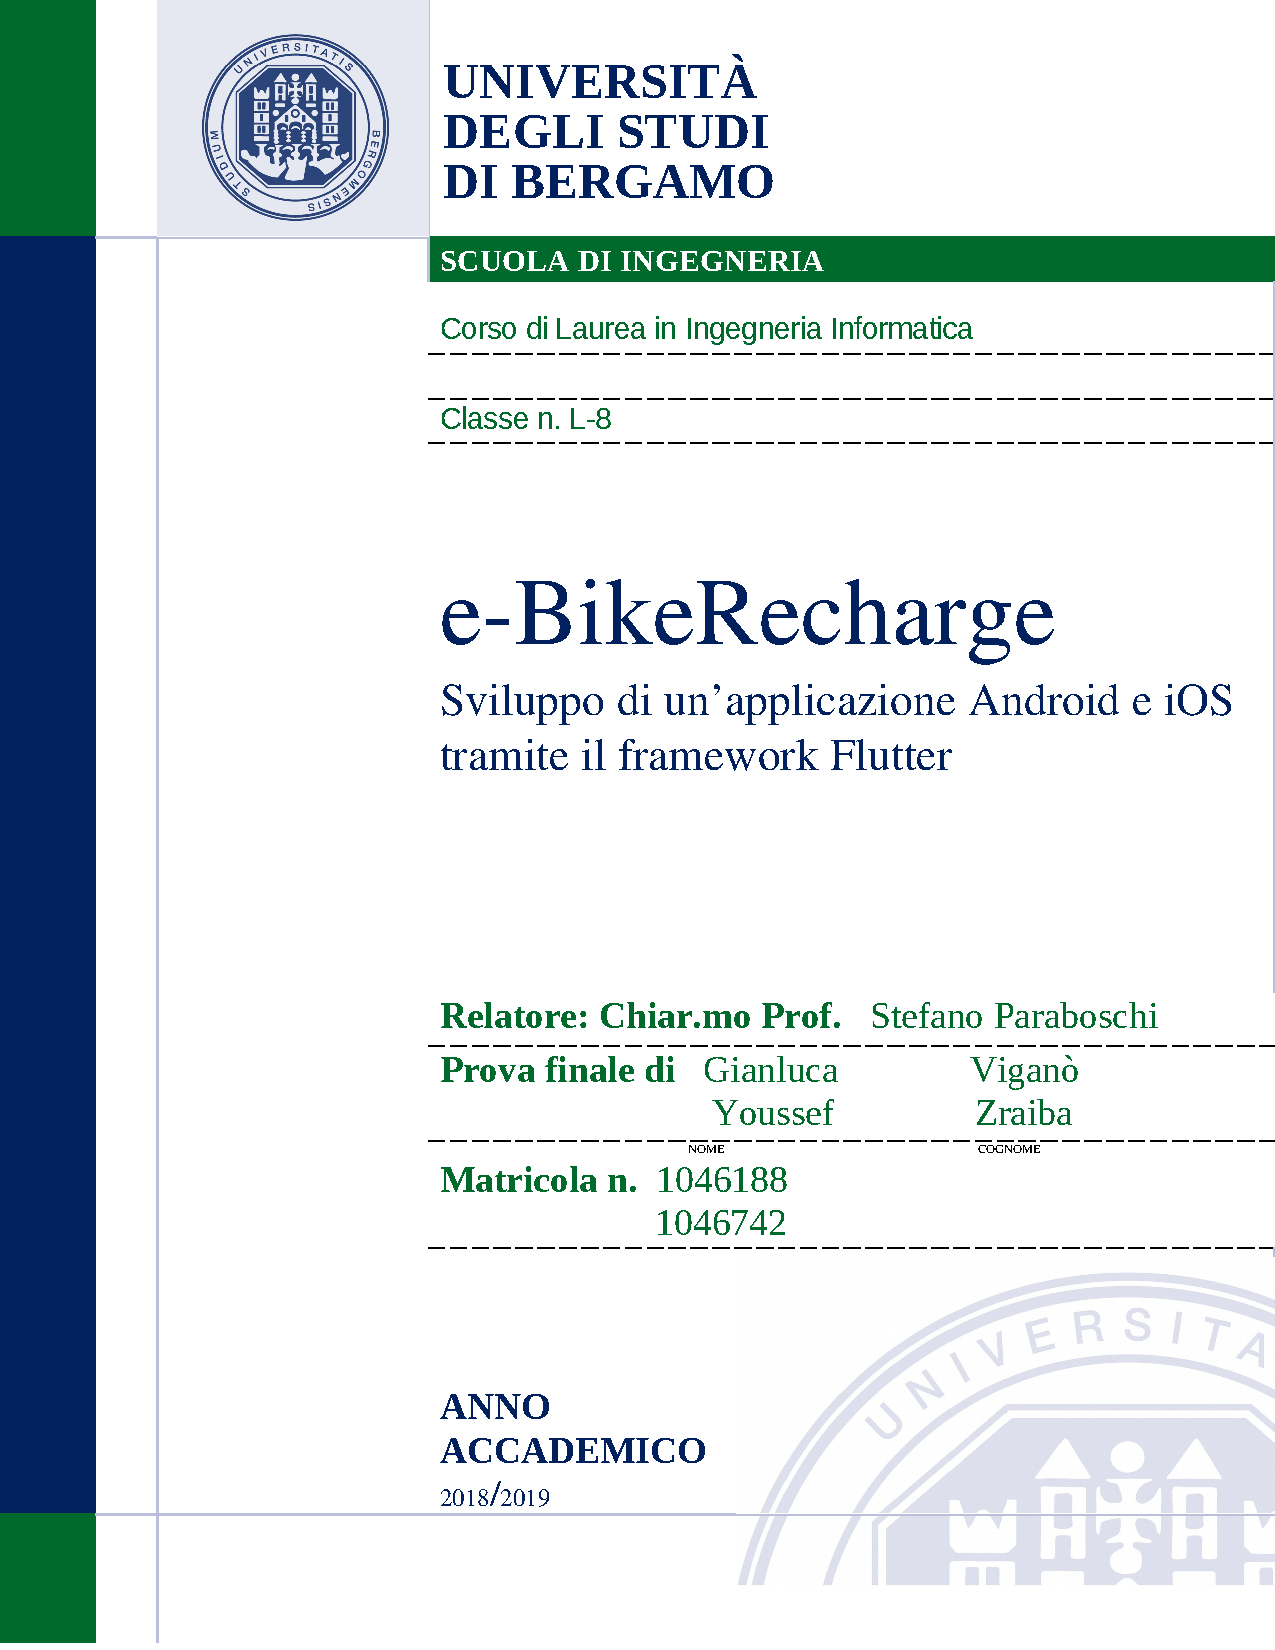
\includepdf[page=-]{copertina2.pdf}
	% \maketitle
	% \newpage
	% Indice
	\tableofcontents
	\newpage
	\pagenumbering{arabic}

	\begin{spacing}{1.5}
	
	% Introduzione
	%\documentclass[../../Tesi.tex]{subfiles}

%\begin{document}

\chapter{Introduzione}
% \section{Introduzione}
	Nel 2017 in Italia la produzione di veicoli a due ruote a pedalata assistita è aumentata
	del 48\% e il mercato dell'e-bike ha ottenuto un incremento del 
	19\%  per un totale di 148.000 unità vendute.
	\cite{biciElettrica}   
	% \subsection{Obiettivi e origine del progetto}
	\section{Obiettivi e origine del progetto}
	Scopo del progetto è creare un’applicazione che mostri all’utilizzatore, in
	base  alla propria posizione, le più vicine stazioni di ricarica per bici
	elettriche. Inoltre vengono forniti numerosi servizi agguntivi per
	facilitarne l'utilizzo e la personalizzazione.\\
	L'idea è nata da un incontro con il dott. Marco Aceti, biker per passione,
	nell'estate 2018. Durante il colloquio ha spiegato come il mercato delle
	bici elettriche sia in continua espansione, e che sempre più ciclisti
	decidono di passare dalla tradizionale bicicletta a quella con pedalata
	assistita. Dunque ha raccontato la sua idea: un'applicazione che mette a
	conoscenza dell'utente la posizione delle colonnine per ricaricare la
	propria bici.
	
	% \subsection{Scelta del framework}
	\section{Scelta del framework}
	Il committente dell'applicazione desiderava che il prodotto fosse 
	usufruibile  da quanti più utenti possibile, e dunque una delle richieste
	era che l'app fosse accessibile sia da dispositivi Apple, con il sistema
	operativo iOS, sia da dispositivi Android. \newline
	Per i sistemi Android non ci sarebbero stati problemi relativi al linguaggio
	da utilizzare in quanto si aveva già avuto esperienza di Java, dei suoi
	costrutti e della sua sintassi. Inoltre il programma Android Studio avrebbe
	ulteriormente semplificato le cose. Il problema nasceva nel momento in cui
	si era deciso di sviluppare un'app per iOS: la nostra conoscenza relativa
	ai
	linguaggi (Swift e C\verb|#|) era pressochè nulla e si sarebbe dovuto
	investire diverso tempo per impararne in modo appropriato l'utilizzo. 
	Inoltre per poter sviluppare un'applicazione che possa poi essere eseguita su un
	Iphone si deve essere in possesso di un calcolatore Apple (Macbook) in
	quanto è necessario il programma Xcode, funzionante solo su quest'ultimo; e
	questo strumento non faceva parte delle nostre risorse.
	Non
	sapendo come procedere, si è deciso di chiedere maggiori informazioni a
	diversi	professori del corso di Ingegneria Informatica e anche al gruppo
	Unibg Seclab. Proprio questi ultimi ci hanno indicato come la soluzione al
	problema fosse un (al tempo) nascente framework di Google in grado di creare
	app native per entrambe le piattaforme di interesse: Flutter. Il prossimo
	capitolo è dedicato alla comprensione e all'utilizzo di concetti base per
	capire come sviluppare software mediante questo framework.
	
	\section{Organizzazione e sviluppo}
	% \subsection{Organizzazione e sviluppo}
	Lavorando in un team è stato necessario impiegare del tempo per scegliere i 
	tool relativi allo sviluppo in gruppo, in modo da organizzare il tutto nel 
	miglior modo possibile.

	\subsection{Git e Bitbucket}
	% \subsubsection{Git e Bitbucket}
	Bitbucket è uno strumento di gestione del codice Git. Un
	progetto sviluppato con questi due tool dunque
	non solo risiede fisicamente sulle macchine sulle quali si testa il
	software, ma anche sul cloud, in modo da avere maggiore affidabilità delle
	versioni (con una gestione efficace relativa alle modifiche) e potendo poi
	accedere con un qualunque calcolatore al progetto. Per aggiungere un nuovo
	file al progetto è necessario scrivere               
	\verb|git --add nomefile|, se invece occore applicare delle modifiche
	inserendo anche un commento per meglio comprendere il lavoro appena concluso
	basta digitare \verb|git commit -a| \verb|-m "messaggio"| (dove il parametro
	\verb|-a| sta a indicare che si vuole applicare a \textit{tutte} le
	modifiche e il parametro \verb|-m| che si desidera lasciare un commento).
	Volendo rendere dunque \textit{effettive} le modifiche è necessario dare
	il comando \verb|git push  origin| \verb|master| in modo tale da inserire nel branch
	\textit{master} la nuova porzione di codice. Per ottenere le modifiche
	aggiunte da un altro membro del team bisogna scrivere \verb|git pull|:
	dopo tale comando sul proprio calcolatore sono presenti tutti i file della
	repository aggiornati all'ultima versione.

	\subsection{Trello}
	% \subsubsection{Trello}
	Trello è un programma che permette in modo molto rapido e soprattutto in
	maniera intuitiva di organizzare le mansioni e i compiti di ogni membro del
	team. La pagina principale consiste in una grande bacheca sulla quale sono
	visibili delle \textit{schede}, ognuna con un titolo e relativa a un
	particolare gruppo. Per ogni scheda è poi possibile indicare il membro del
	team al quale è riferito il lavoro indicato, indicare una lista di azioni
	(in modo da vedere la percentuale di avanzamento di quella particolare
	scheda) e settare dei promemoria importanti che non devono essere persi.

	\subsection{Visual Studio Code}
	% \subsubsection{Visual Studio Code}
	Il progetto conteneva numerosi file di estensione diversa. Infatti erano
	presenti file dart (per l'applicazione vera e propria), xml (per lavori
	specifici lato Android), plist (file descrittivo lato iOS), immagini e altri
	ancora. Si è quindi deciso di utilizzare un editor testuale il più generale
	possibile e non legato allo sviluppo di un particolare linguaggio. La
	scelta è ricaduta su Visual Studio Code, di proprietà Microsoft. Oltre a
	possedere "out of the box" funzionalità molto comode per lo sviluppo
	software, è estensibile con migliaia di pacchetti relativi a pressochè ogni
	linguaggio. Nello specifico l'estensione per Flutter non solo presenta
	autocompletamenti vari e molto dettagliati, ma anche una comoda funzione per
	fare il debugging del software gestendo il tutto con una barra che raccoglie i
	principali comandi. 

	\section{Struttura generale dell'applicazione}
	% \subsection{Struttura generale dell'applicazione}
	Di seguito viene riportato un accenno alla struttura, alle pagine
	dell'intera applicazione in modo da dare un contesto e dare una visione
	d'insieme al lettore. A partire dal terzo capitolo ogni pagina verrà poi
	analizzata nel dettaglio in base ai propri componenti e alle sue
	funzionalità, mostrando anche immagini e codice. \newline
	Al primo accesso all'utente viene mostrata una pagina di login nella quale
	si può inserire la propria mail e password oppure creare un nuovo account.
	Se l'autenticazione o la creazione di un nuovo utente sono andate a buon
	fine, viene mostrata la pagina principale, la mappa, che indica tutte le
	stazioni di ricarica, noleggio e manutenzione di bici elettriche presenti
	nel database. Oltre a possedere numerose funzioni che verranno descritte nel
	proprio capitolo, da questa pagina è possibile accedere all'inserimento di
	una nuova stazione (che deve essere in ultimo confermata del gestore del
	database), e si può infine arrivare alla pagina profilo, dove si possono
	settare impostazioni personali come la tipologia di mappa che si vuole
	visualizzare e cambiare la password, si possono vedere le stazioni aggiunte
	dall'utente attuale ed effettuare il logout, per tornare così alla pagina
	iniziale di login. 	
	
%\end{document}
	% capitoli
	\newpage
	% \section{Sistemi Operativi per smartphone: \\ Android e iOS}
\chapter{S.O. per smartphone:\\Android e iOS}
L'applicazione è stata realizzata tramite il framework Flutter (a cui sarà
dedicato l'intero prossimo capitolo), in modo tale da poter sviluppare lo stesso
progetto per i due maggiori sistemi operativi per smartphone: Android di
proprietà di Google e iOS dell'azienda Apple. In questo capitolo si prendono in
considerazione tali sistemi focalizzandosi soprattutto sul funzionamento.

\section{Android}
% \subsection{Android}
Android è un sistema operativo mobile, realizzato per dispositivi mobili
touchscreen, ed è stato sviluppato inizialmente dall'azienda Android Inc., che
nel 2005 è stata acquistata da Google \cite{3}.\\
Una delle caratteristiche più importanti di questo sistema operativo è che 
detiene una licenza open source. Questo tipo di licenza consente a
qualsiasi utente di modificare e distribuire liberamente il codice
sorgente, consentendo quindi una continua evoluzione del sistema operativo e una
più semplice diffusione. Considerando i processi, Android riesce a gestirli in
modo da mantenere il consumo energetico al minimo. Quando un’applicazione non è
in uso, il sistema sospende il suo funzionamento ma allo stesso tempo la rende
disponibile per l’uso immediato, così che l’applicazione non contribuisca
al consumo della batteria. Il sistema operativo gestisce le applicazioni archiviate in
memoria, in modo tale che sull'esaurirsi della memoria volatile il sistema inizi
automaticamente a chiudere i processi, partendo da quelli che sono rimasti
inattivi per il periodo di tempo più lungo.

\subsection{Kernel Linux e Architettura}
% \subsubsection{Kernel Linux e Architettura}
Un kernel può essere considerato come un ponte tra hardware e software, e può comunicare con
l’hardware tramite i driver che sono inclusi al suo interno. In questo modo, quando
un’applicazione vuole rispondere a un comando, può inoltrare le istruzioni al
kernel e quest’ultimo può utilizzare i driver dell’hardware che si vuole
controllare per ottenere il comportamento desiderato. In particolare, Android si
appoggia al kernel Linux. Esso fornisce
tutte le funzioni essenziali per il sistema, tra cui la gestione della memoria
primaria e la gestione delle risorse hardware del sistema e delle periferiche.
Il suo incarico quindi è quello di gestire
il tempo processore, le comunicazioni e la memoria, assegnando ogni cosa ai processi in
corso in base alle priorità assegnate. Il kernel Linux è adatto a tutte quelle
tecnologie embedded più rilevanti, e quindi ha avuto molto successo nel campo
delle tecnologie portatili.
Esso è inoltre utilizzato dal sistema operativo Android, sebbene Google abbia
introdotto qualche variazione. Una di queste è la funzionalità di gestione
del risparmio, chiamata \textit{wakelocks}, che impedisce al telefono di lavorare a
basso consumo. Nel kernel Linux non c’è un’implementazione completa della
Libreria Standard del linguaggio C++ (STL), dato che le applicazioni Android si
basano sul linguaggio di programmazione Java. Da questo segue che per svolgere
la propria funzione tutte le chiamate a
sistema fatte in C/C++ devono richiamare la Java Virtual Machine. Oltre al
kernel Linux, Android è formato anche da  middleware, Librerie e API scritte in
C/C++ (fig. \ref{kernel}). Le
ultime versioni di Android usano ART Virtual Machine, mentre nelle vecchie versioni
veniva utilizzata la Dalvik Virtual Machine (entrambe considerate nel prossimo
paragrafo).
\begin{figure}
    \centering
    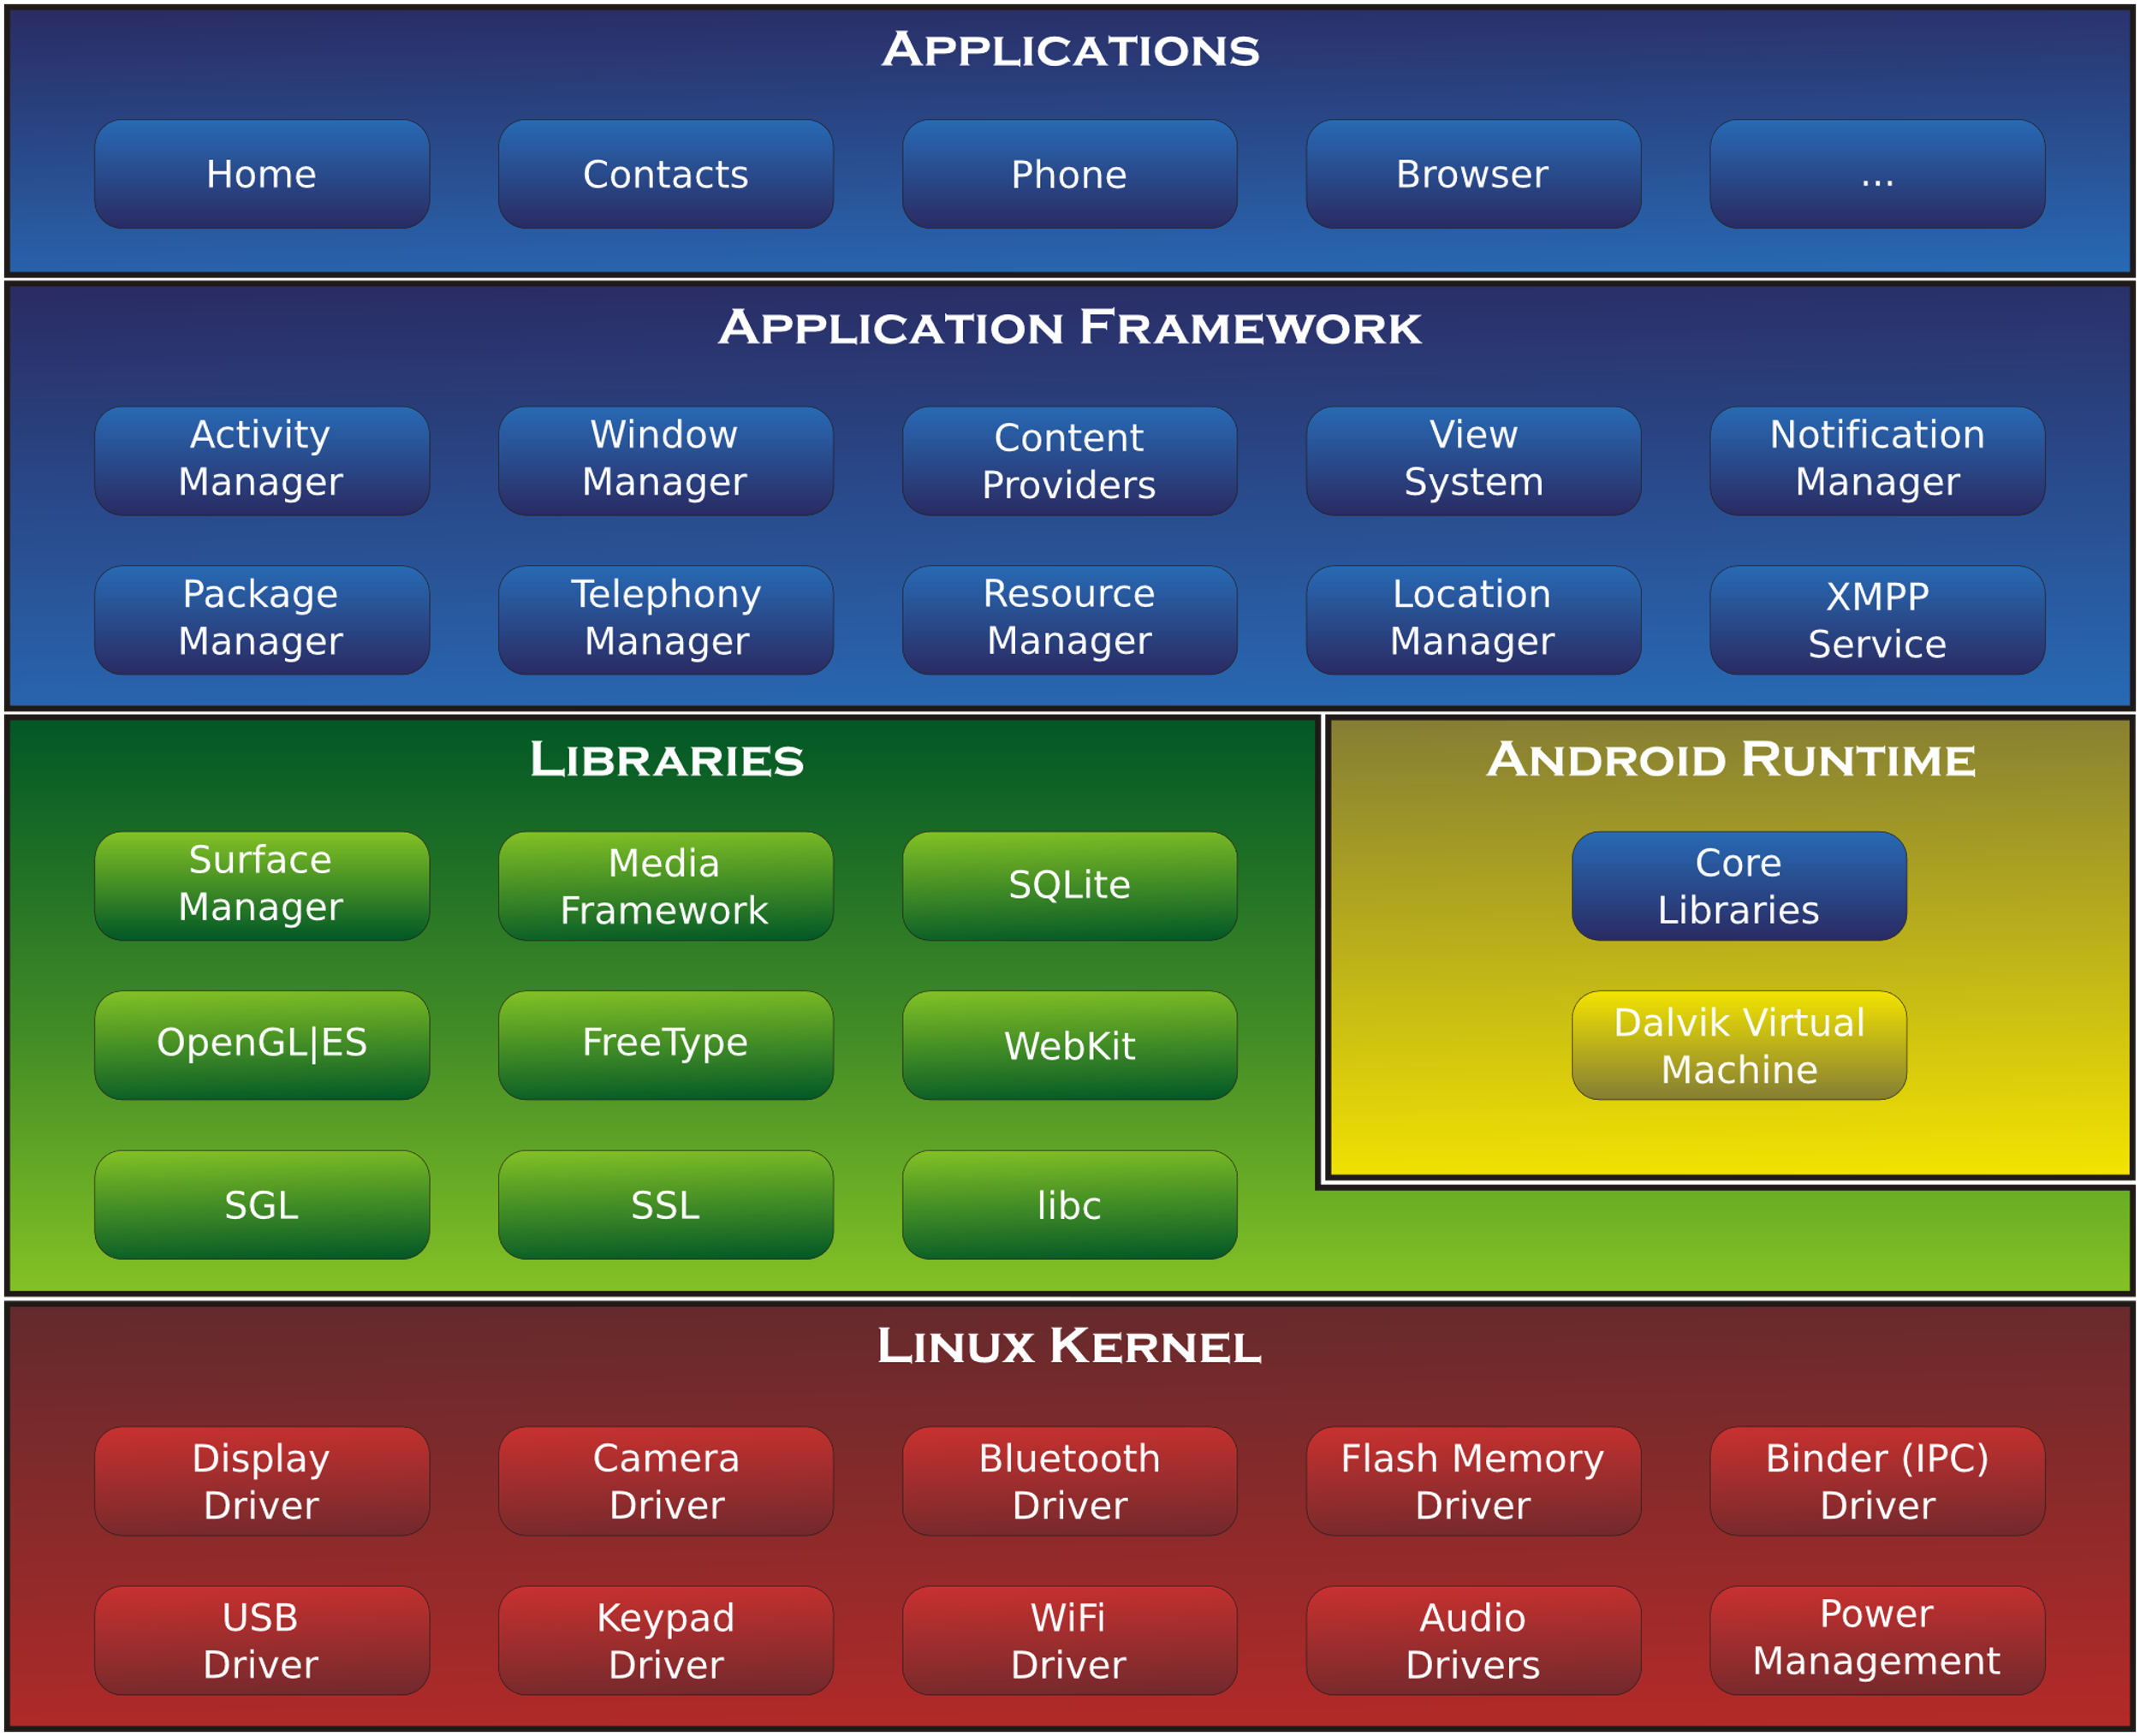
\includegraphics[width=9.5cm]{kernel.png}
    \caption{Struttura del sistema operativo Android \cite{4}}
    \label{kernel}
\end{figure}

\subsection{ART Virtual Machine e Dalvik Virtual Machine}
% \subsubsection{ART Virtual Machine e Dalvik Virtual Machine}
La VM, Virtual Machine, è in Android il software all’interno del 
quale vengono eseguite le applicazioni. Le applicazioni Android vengono scritte in
linguaggio Java, il quale viene poi compilato in Bytecode
(intermedio tra il linguaggio macchina e il linguaggio di
programmazione che permette che il codice possa essere eseguito su macchine
diverse con hardware diversi), compilato infine
dalla Virtual Machine. Inizialmente in Android veniva utilizzata la Dalvik VM,
che a partire dalla versione 4.4 KitKat di Android, è stata sostituita dalla ART
VM.
La VM Dalvik è basata su tecnologia \textit{just-in-time}: ogni applicazione viene
compilata solo in parte dal programmatore e sarà poi di volta in volta dovere
della Dalvik VM eseguire il codice e compilarlo in linguaggio macchina in tempo
reale. Questo ovviamente grava sulle prestazioni.
La ART VM (Android Run Time) invece è basata su tecnologia \textit{ahead-of-time} che esegue l'intera
compilazione del codice durante l'installazione dell'applicazione e non durante
l'esecuzione stessa del software. Questo permette di avere un vantaggio in
termine di prestazioni, anche se incide sul tempo di installazione delle
applicazioni.

\subsection{Sviluppo applicazioni in Android}
% \subsubsection{Sviluppo applicazioni in Android}
In aiuto ai programmatori per la scrittura di applicazioni Android esiste un
kit di sviluppo software  chiamato SDK. L’SDK  comprende un numeroso set di
strumenti di sviluppo, tra cui: librerie software, debugger, documentazione e
codice d’esempio. Esistono poi diversi ambienti per lo sviluppo, tra questi si
ricordano Visual Studio Code, Atom, Eclipse e Android Studio. Quest'ultimo è considerato l'IDE
primario per lo sviluppo di applicazioni, in quanto presenta notevoli agevolazioni.
I progetti Android sono costituiti da parti dinamiche scritte in Java e
parti statiche scritte in XML. L’SDK permette  di eseguire le applicazioni sia
in emulazione, sia su un dispositivo vero e proprio. Per descrivere
l’applicazione allo smartphone che si vuole utilizzare, si fa ricorso al file
Manifest.xml, questo elenca la lista delle necessità del software per poter
funzionare in modo adeguato. Per motivi di sicurezza, per evitare che
applicazioni di terze parti abbiano i permessi per poter accedere a informazioni
private all’interno del
telefono, bisogna controllare attentamente il contenuto del Manifest, e non
installare il software in caso richieda risorse non coerenti con lo scopo
dichiarato dell’applicazione. Una volta scritta e concluso il progetto, il
codice java e il codice XML vengono compilati generando un file con estensione
.apk (l’eseguibile delle applicazioni Android). Esso contiene il bytecode che verrà
eseguito dalla Virtual Machine. Le applicazioni Android sono pilotate
dagli eventi (Event Driven), causati da hardware o da altri
componenti. Il programmatore quindi sviluppa per ogni hardware routine
indipendenti, permettendo al sistema operativo di rinunciare al caricamento di
componenti che non si andranno a utilizzare, facendo uso solo di quelli che sono
strettamente necessari. \\
Quando si avvia per la prima volta un dispositivo Android, si può notare come su
tale sistema siano già presenti
applicazioni di terze parti, che possono essere utilizzate fin da subito
dagli utenti. Quando si vuole utilizzare un'applicazione non ancora presente sul
proprio smartphone bisogna scaricare e installare il file apk dell’applicazione
dal Google Play Store. Quest’ultimo è il principale "negozio" di
applicazioni installato su dispositivi Android, e consente agli utenti di
scaricare e aggiornare le applicazioni pubblicate da Google o sviluppatori di
terze parti. Esistono infine anche un certo numero di store di app di terze
parti, che forniscono servizi che non possono essere offerti dallo store
ufficiale a causa di violazioni di particolari norme.

\section{iOS}
% \subsection{iOS}
Il sistema operativo creato da Apple è esclusivo dei propri device, in quanto
solo gli iPhone presentano questo software poichè l'azienda, a differenza di
Android, non concede licenze per l’installazione di iOS su hardware diverso da quello
proprietario. Nonostante questo aspetto è però il secondo
sistema operativo mobile più popolare al mondo \cite{rep}. \\
Per lo sviluppo di queste applicazioni viene messo a disposizione un SDK apposito,
disponibile unicamente per PC Mac. L’SDK contiene diversi strumenti che
consentono ai programmatori di utilizzare le varie funzioni e servizi dei
dispositivi iOS. Il Software Development Kit, in coppia con XCode, assiste gli
sviluppatori durante il processo di sviluppo dell'applicazione utilizzando
linguaggi di programmazione ufficialmente
supportati (Swift
e Objective-C). Xcode è un ambiente di sviluppo per macOS adibito allo sviluppo
di software in grado di essere esguito sui dispositivi dell'azienda di
Cupertino. La suite Xcode include la maggior parte
della documentazione per sviluppatori di Apple e con un Interface Builder integrato,
(applicazione facile e intuitiva utilizzata per costruire interfacce utente
grafiche) Al suo interno è anche presente un simulatore in grado di creare un
iPhone virtuale all'interno del proprio Mac su cui poi testare le applicazioni
sviluppate.
\subsection{Architettura}
% \subsubsection{Architettura}
Le app interagiscono con l’hardware attraverso una serie di interfacce di
sistema. Queste interfacce semplificano la scrittura di applicazioni per i
dispositivi Apple. I livelli inferiori forniscono servizi di base a cui tutte le
applicazioni fanno affidamento, quelli superiori invece forniscono servizi
per avere una grafica di alto livello. iOS usa kernel XNU (\textit{X is Not
Unix}) ed è caratterizzato da
4 livelli di astrazione: il Core OS Layer, il Core Services Layer, il Media layer e
il Cocoa Touch Layer (fig. \ref{ios1}). Ogni livello ha una serie di framework
utilizzabili dagli sviluppatori. 
\begin{figure}[!h]
    \centering
    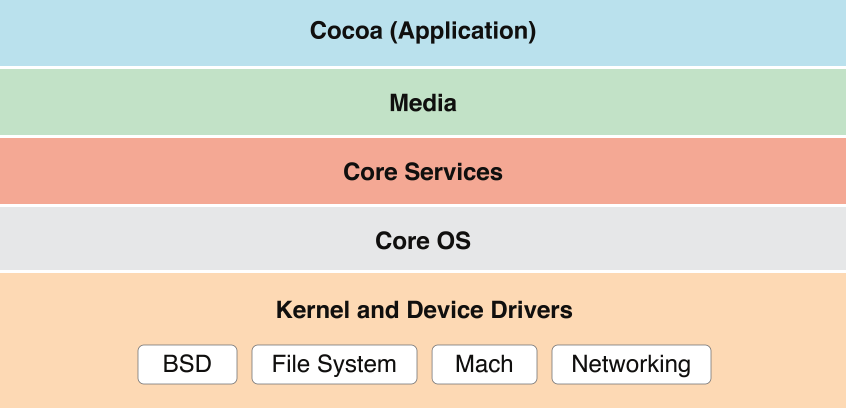
\includegraphics[width=9cm]{ios1.png}
    \caption{Struttura del sistema operativo iOS \cite{huhuh}}
    \label{ios1}
\end{figure}

Il livello più basso di iOS è costituito dal kernel di cui si parlerà nel
prossimo paragrafo. Al di sopra del kernel, si ha il Core OS,
responsabile della gestione della memoria, delle attività del file system, della
rete e delle attività del sistema operativo ed interagisce anche con l’hardware.
Al livello successivo è presente il Core Services, il quale fornisce servizi Peer-to-Peer,
archiviazione su iCloud, protezione dati, supporto per condivisione di file, Grand
Central Dispatch, SQLite, supporto XML e gestisce anche gli acquisti in app. Successivamente
si ha il Media Layer, che fornisce al sistema operativo funzionalità audio, video
e animazioni. L’ultimo livello, il Cocoa Touch, contine framework molto importanti
che definiscono l’aspetto dell’app. Esso fornisce anche l'infrastruttura di base delle
applicazioni e supporto per tecnologie importanti come multitasking, touch,
notifiche push e per altri aspetti di alto livello.

\subsection{Kernel XNU}
% \subsubsection{Kernel XNU}
Il kernel XNU, come detto precedentemente, fa da mediatore tra il software
e l’hardware, ed è il primo programma ad essere caricato in memoria
all’accensione del dispositivo. XNU è utilizzato nel sistema operativo open source
Darwin, ed Apple lo usa come base per il proprio software. Esso è inoltre
ibrido, poiché formato da due tipologie di kernel: il microKernel Mach e il
Kernel BSD (fig. \ref{ios2}).
Inoltre XNU è modulare, ovvero è possibile utilizzare moduli aggiuntivi
attivabili e disattivabili durante il funzionamento. \\
Il primo componente, il vero e proprio cuore di XNU, è Mach, microkernel che gestisce le
responsabilità elementari del sistema operativo: scambio di messaggi tra
processi, pianificazione delle attività, gestione della memoria virtuale ed
elaborazione dei thread. Il secondo componente è il kernel BSD, che fornisce un
livello di astrazione superiore e permette l’accesso ai dispositivi e al file
system. L’ultimo componente è il framework I/O Kit, completamente indipendente
dal kernel e consente agli sviluppatori di creare rapidamente driver per i
dispositivi. \\
\begin{figure}[!h]
    \centering
    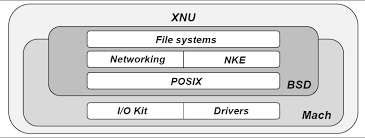
\includegraphics[width=11cm]{ios2.png}
    \caption{I diversi livelli e sezioni del kernel XNU \cite{xnu}}
    \label{ios2}
\end{figure}



	\newpage
	\section{Flutter}
	I pregi di Flutter sono numerosi e se ne vogliono citare alcuni. \newline
	Per primo si considera il linguaggio. Flutter viene sviluppato con il
	linguaggio (sempre appartente alla famiglia Google) Dart. Esso è
	multifunzione, può essere impiegato per lo sviluppo web (tant'è che è nato
	 per sostituire Javascript) e in tale linguaggio una variabile può sia
	presentare una tipazione statica a compile time, sia essere definita
	\textit{dynamic} e cambiare tipo più
	volte nel corso dell'esecuzione. Con Flutter basta scrivere una volta sola
	il proprio codice in Dart, e il framework penserà poi a creare i file
	necessari per essere eseguiti sia su iOS che su Android. Da qui ne segue un
	enorme risparmio di tempo e risorse, in quanto si dimezza il lavoro totale.
	Un altro aspetto importante è che
	grazie ad esso è possibile sviluppare in modo rapido, e ciò è permesso dalla
	funzione \textit{Hot Reload} che consente in qualche secondo di ricaricare
	la particolare sezione di codice che si sta testando senza dover ricaricare
	l'intera applicazione. In secondo luogo tale framework presenta
	facilitazioni notevoli relative al design degli elementi: con poche righe e
	senza essere esperti di grafica si può creare qualcosa dall'aspetto tutt'altro che
	banale. \'E doveroso accennare anche alle prestazioni: i \textit{widget}
	(elementi) di Flutter gestiscono automaticamente l'implementazione di
	funzionalità comuni quali lo scrolling, la navigazione, le icone e i
	caratteri in
	modo da rendere le performance del software paragonabili a quelle di app
	native sia su iOS sia su Android. 

	\subsection{Stateless e Statefull Widget}
	In Flutter esiste una prima importante distinzione fra widget diversi:
	quelli \textit{senza stato} e quelli \textit{con stato}. I primi possono
	anche essere chiamati widget statici, in quanto la loro forma non varia
	durante l'esecuzione. Nell'immagine \ref{stateless1}  viene mostrato un esempio di widget
	stateless. Innanzitutto bisogna importare il pacchetto
	\textit{flutter/material.dart} che contiene tutti i principali widget. Nel
	metodo main è presente solo una funzione, denominata \textit{runApp}, che
	ottenuto in input un widget con particolari caratteristiche, esegue sul
	dispositivo di test tale widget. Nell'esempio esso è chiamato MyApp ed
	estende la classe StateLessWidget. Un oggetto di questo tipo deve
	sovrascrivere il metodo \textit{build} che riceve in input il contesto nel
	quale l'app si trova (che consiste nel particolare valore delle variabili e
	di altri oggetti in quel preciso istante di esecuzione), e ritorna il widget
	vero e proprio che dovrà essere eseguito. Per ottenere una corretta
	struttura, anche in progetti più complessi di questo semplice esempio, è
	necessario introdurre la classe MaterialApp, e tramite il suo costruttore
	definire la sua \textit{home}, cioè la pagina principale, con una Scaffold,
	definibile come l'impalcatura del widget. \'E necessario introdurre nel parametro
	\textit{body} la classe che si vuole eseguire, la quale a sua volta estende
	StateLessWidget e presenta ancora il metodo build. Qui viene ritornato un
	widget che avrà posizione centrale (Center), sarà contenuto in un
	contenitore (Container, utile per decorare e aggiungere funzionalità a
	specifiche sezioni di codice), e mostrerà un testo con il più classico dei
	messaggi d'avvio (Hello World!). Questo widget non è interattivo, non
	cambierà mai graficamente e perciò si dice che non ha stato.
	 Da questo esempio si può già notare come la
	struttura del codice flutter assuma \textit{graficamente} un'indentazione
	naturale, con una gerarchia ad albero in cui c'è un padre iniziale e da cui
	seguono numerosi figli, padri di successivi widget.

	\begin{figure}[h!]
		\centering
		\begin{subfigure}{0.6\linewidth}
			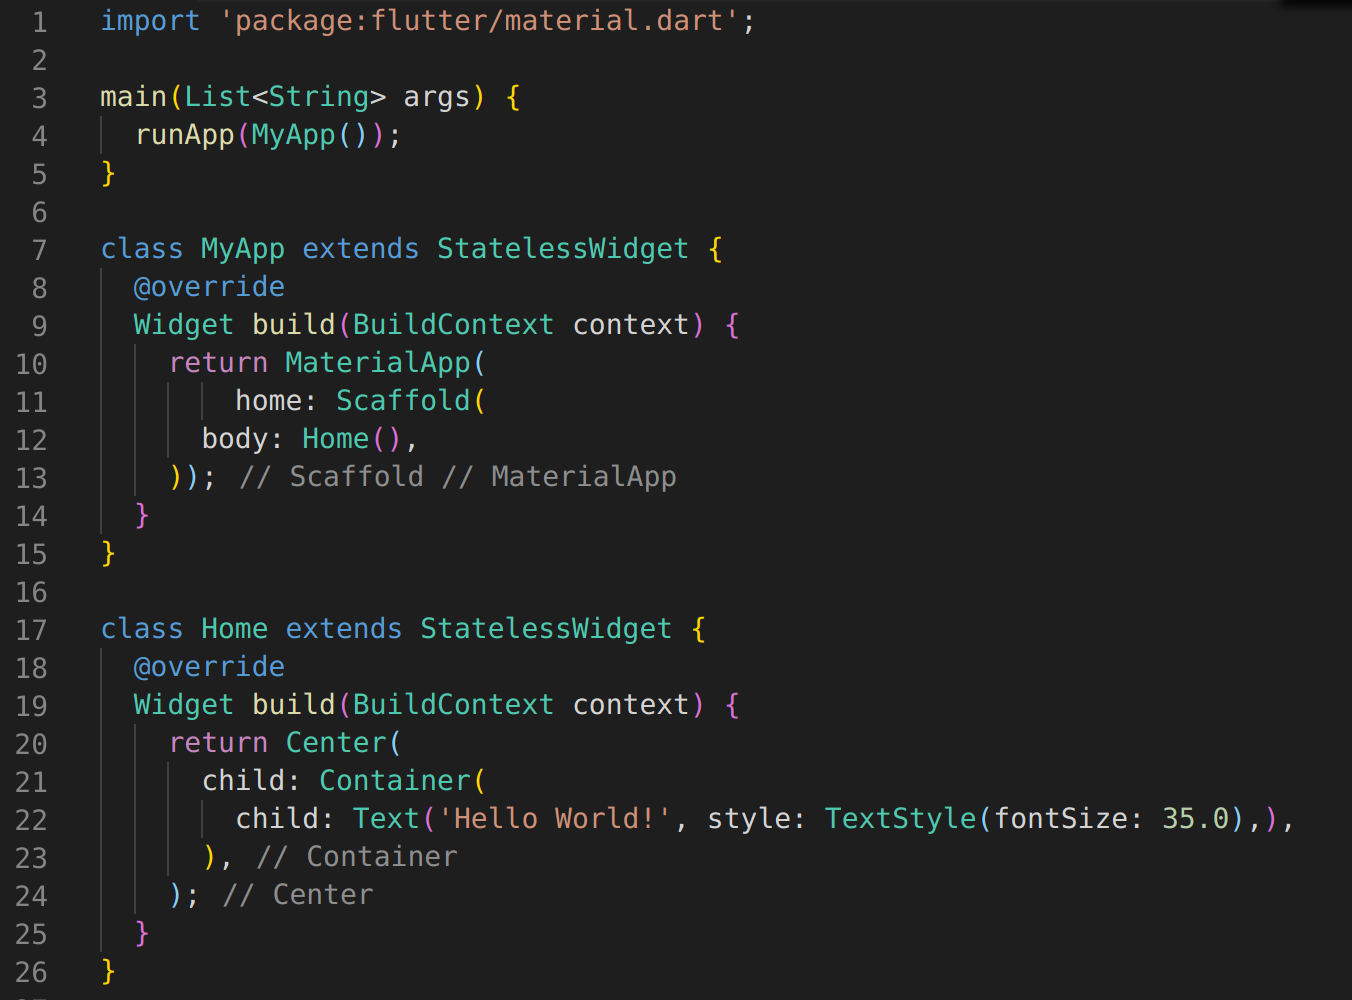
\includegraphics[width=\linewidth, height=7cm]{StateLessApp.png}
			\caption{Esempio di codice di widget stateless}
		\end{subfigure}
		\begin{subfigure}{0.3\linewidth}
			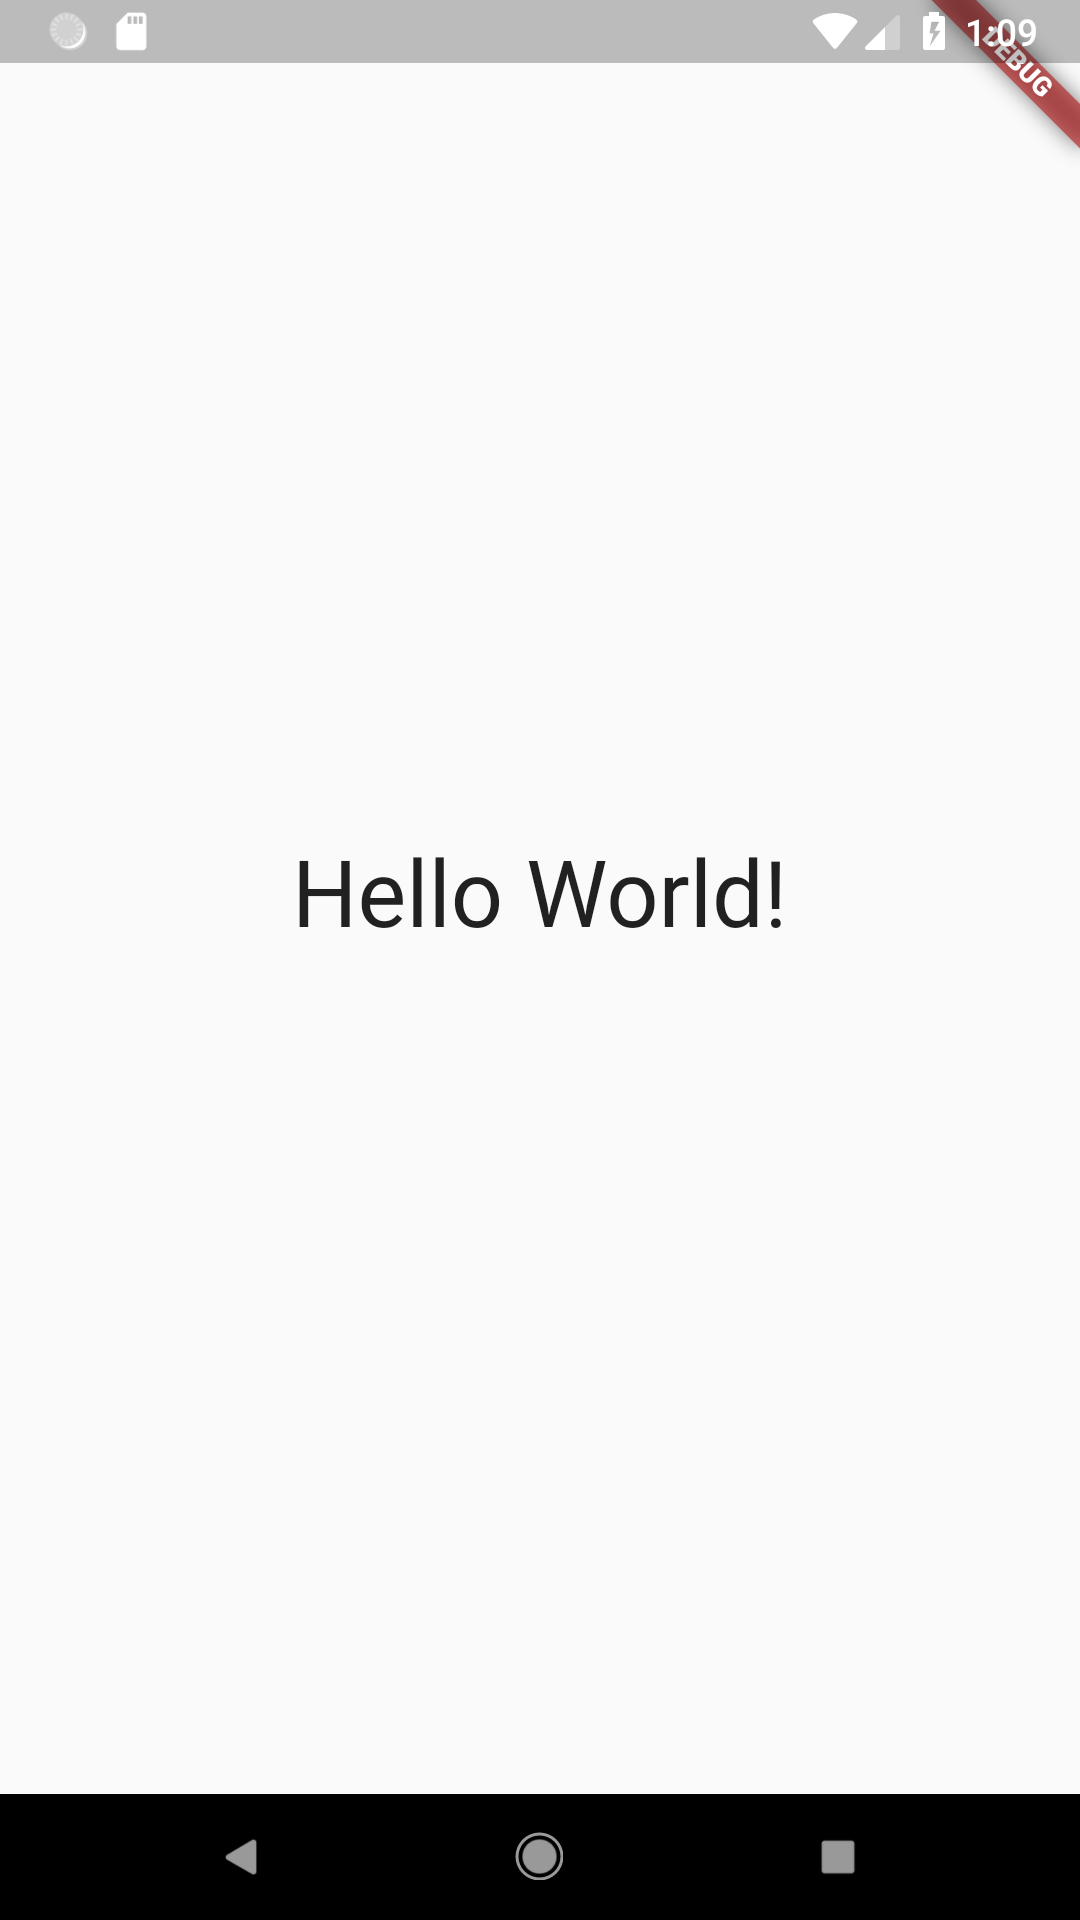
\includegraphics[width=\linewidth, height=7cm]{StateLessScreen.png}
			\caption{Risultato}
		\end{subfigure}
		\caption{}
		\label{stateless1}
	\end{figure} 

	Nell'immagine \ref{statefull} viene mostrato invece un widget di tipo
	Statefull. Si può notare come la prima parte del codice sia identica, con la
	classe MyApp che è ancora un widget senza stato. Ciò che cambia è la classe
	Home che ora è con stato e presenta un unico metodo sovrascritto chiamato
	\textit{createState}. La freccia =$>$ in dart è una notazione per scrivere in
	modo compatto un metodo che ritorna un unico oggetto, in questo caso una
	classe chiamata \_HomeState, che estende State$<$Home$>$. Il trattino basso
	in dart sta a indicare un oggetto privato, a cui quindi non è possibile
	accedere se non in quella specifica classe. \_HomeState possiede una
	varibile di tipo intero denominata counter (anch'essa privata grazie al
	trattino basso) e ha valore iniziale 0. Presenta poi un metodo denominato
	buttonPressed al cui interno risiede una funzione molto importante, la
	\textit{setState}. Quando viene compliata una sezione di codice che sta
	all'interno di tale funzione, viene richiamata la funzione build del widget
	in esecuzione ed è quindi grazie ad essa che l'app diventa interattiva, in
	quanto tramite azioni dell'utente cambiano i valori delle variabili.
	Nell'esempio è presente un pulsante (FloatingActionButton) che aumenta il
	valore della variabile counter, che viene stampato a schermo. Da notare
	infine come si possa accedere al metodo toString di un oggetto in dart
	anteponendo al suo nome il carattere \$.

	\begin{figure}[h!]
		\centering
		\caption{Esempio di codice di widget statefull}{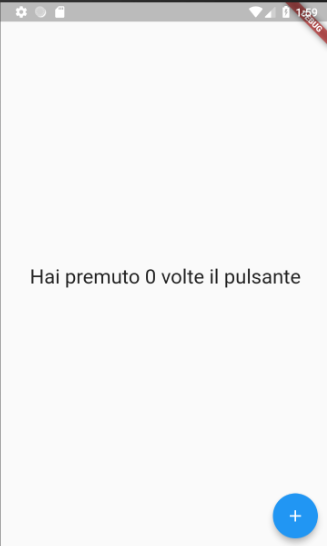
\includegraphics[scale=0.35]{StateFullApp.png}\label{statefull}}
	\end{figure}

	\subsection{Principali Widget}
	Di seguito vengono riportati i widget di cui si è fatto maggiore uso
	all'interno dell'applicazione.
	
	\begin{trivlist}
		\item \textbf{Text} \newline
		Questo widget permette di mostrare a schermo le stringhe fornite come
		primo argomento al suo costruttore (\verb|Text("Testo da mostrare")|).
		Il testo può svilupparsi su più righe o su una sola a seconda delle
		costanti di layout della particolare schermata nella quale risiede il
		widget. Nel costruttore possono essere indicati diversi argomenti
		opzionali, tra cui lo stile. Se si vuole indicare un particolare stile
		al proprio testo bisogna inserire un TextStyle, cioè un'ulteriore classe
		che gestisce il font, l'inserimento del grassetto o del corsivo e la
		formattazione dell'intero testo (giustificato, allineato a sinistra o a
		destra e centrale).  
		\item \textbf{Row, Column} \newline
		Questi widget vengono spesso utilizzati per ottenere schermate ordinate
		e gradevoli dal punto di vista estetico all'utilizzatore. Il parametro
		principale di entrambe è l'argomento \verb|children| (e non \verb|child| come
		spesso accade per altre classi), proprio perchè sono pensati per
		contenere diversi widget disposti rispettivamente in orizzontale o in
		verticale. La loro grandezza in pixel sarà formata dalla somma della
		dimensioni di ciò che contengono e si possono ancora una volta inserire diverse
		preferenze di stile come la posizione rispetto all'asse principale o
		secondario. 
		\item \textbf{Stack} \newline
		\'E simile ai due precedenti in quanto anch'esso contiene diversi widget
		figli. Se ne differenzia in quanto non privilegia un'unica direzione di
		posizionamento, ma si può indicare per ogni figlio la posiziona esatta
		in pixel che dovrà avere sullo schermo. Questo passaggio viene
		effettuato racchiudendo il widget che si vuole inserire all'interno di
		un'istanza della classe Positioned (che sarà uno dei figli dello Stack)
		e indicando gli esatti pixel nel suo costruttore. 
		\item \textbf{Container} \newline
		Crea un elemento rettangolare che avrà come altezza e lunghezza le
		minime dimensioni per poter contenere il widget indicato come child. \'E
		molto utilizzato nel momento in cui si vuole migliorare graficamente una
		schermata in quanto tramite il parametro opzionale decoration si può
		introdurre una nuova classe chiamata BoxDecoration che gestisce un
		grande insieme di aspetti grafici come i contorni (angoli e
		ombre) o riempire con un colore o un'immagine il Container.
	\end{trivlist}

	\subsection{Material Design}
	Il Material Design è un linguaggio visuale che unisce i classici principi di
	un buon design con l'innovazione della tecnologia e della scienza. 
	\cite{material} \newline
	Tale design è interamente sviluppato da Google e fa uso di layout basati su
	una griglia, animazioni e transizioni. Sono
	

	\newpage
	\chapter{Gestione degli utenti}
% \section{Gestione degli utenti}
Per gestire al meglio la procedura di autenticazione dell'applicazione, la
registrazione e le preferenze dei singoli utenti, si è scelto di utilizzare
Firebase, servizio di database basato sul cloud appartenente a Google.

\section{Firebase}
% \subsection{Firebase}
Firebase è un ottimo servizio di backend che rende disponibili, tramite API,
numerosi servizi tra cui lo storage dei dati, l'autenticazione, notifiche push e
molto altro. Una delle caratteristiche più utili di questo servizio è la
capacità di sincronizzazione dei dati oltre che di storage: le informazioni
vengono infatti aggiornate pressochè all'istante, a patto che l'app web o mobile
sia collegata alla rete. Inoltre sono disponibili numerose librerie client che
rendono ancora più semplice l'integrazione con il proprio prodotto software.
Anche la sicurezza ha un aspetto rilevante, in quanto i dati immagazzinati sono
replicati e sottoposti continuamente a backup e la comunicazione con il client
avviene in modalità crittografata tramite SSL con certificati a 2048 bit.
Esistono tre piani tariffari per utilizzare Firebase. Il primo, gratuito, è
chiamato Spark e comprende i servizi base, tra cui l'autenticazione, fino a 100
connessioni simultanee, 1 GB totale di spazio per i dati e 5 GB per lo storage
di immagini e file. Il secondo è il Flame Plan nel quale aumentano i limiti (50
GB per lo storage e fino a 2,5 GB per i dati) al costo di 25\$ al mese.
L'ultimo è il Blaze Plan nel quale ogni servizio possiede un costo unitario
relativamente basso e funziona con una politica \textit{pay as you go}. Per le
esigenze del progetto le funzionalità offerte da Spark sarebbero state
sufficienti.

\section{Schermata di avvio, tipologia di Utente e pagina Profilo}
% \subsection{Schermata di avvio, tipologia di Utente e pagina Profilo}
Nella schermata d'avvio (figura \ref{login}) l'utente può scegliere di accedere
all'applicazione in tre modi diversi: tramite accesso standard (utente
standard), tramite il pulsante \textit{Accedi con Google} (utente Google) o
tramite accesso anonimo. A seconda della tipologia, le pagine accessibili
cambiano, così come i servizi disponibili.
\begin{figure}[h!]
    \centering
    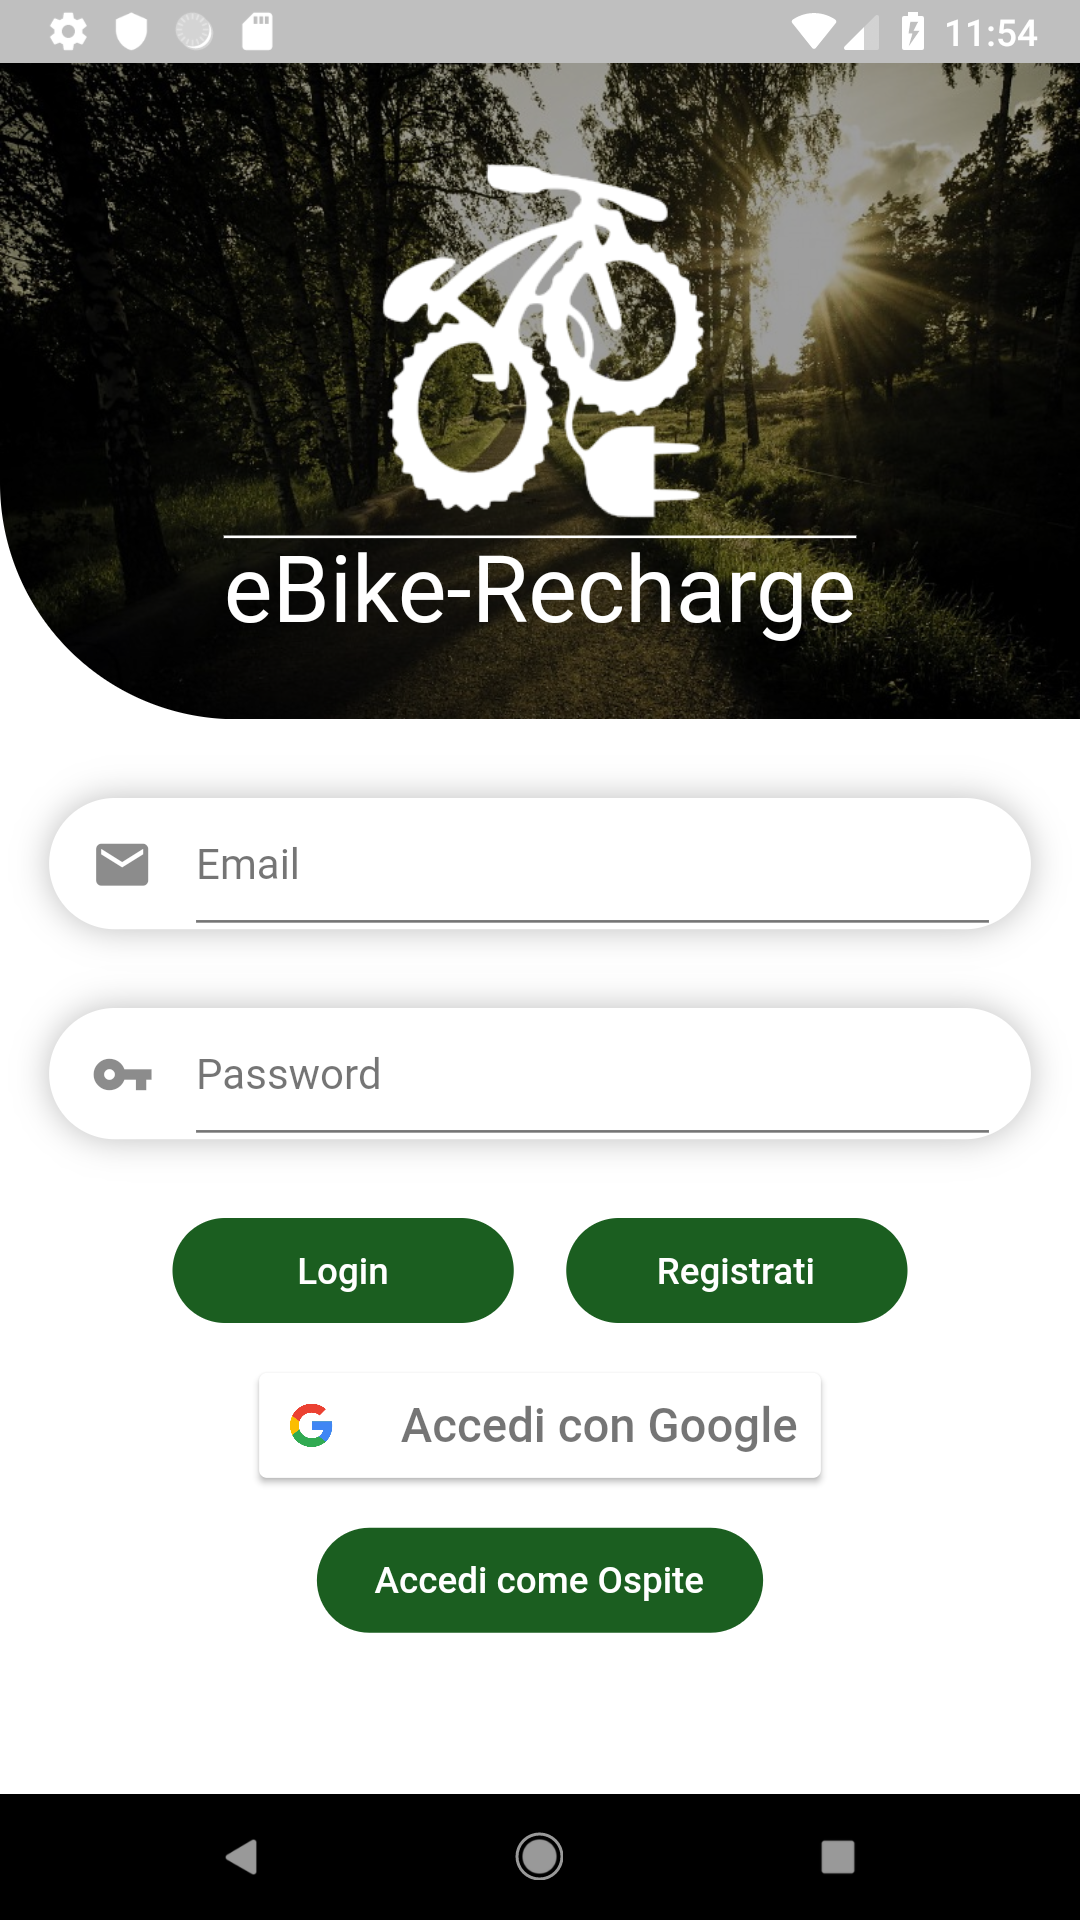
\includegraphics[scale=0.15]{Login.png}
    \caption{Schermata d'avvio}
    \label{login}
\end{figure}
Se l'utente è gia registrato in modo standard, può inserire la propria mail
(usata come username) e la propria password. Se i dati forniti combaciano con
quelli presenti nel database degli utenti si fa accesso alla pagina della mappa
che verrà descritta in un prossimo capitolo. Se invece non c'è corrispondenza
con un utente già registrato viene mostrato a video un messaggio di errore che
mostra in modo chiaro e comprensibile quale sia il problema. \newline
Si può anche fare accesso all'applicazione utilizzando i servizi Google che
permettono di autenticarsi mediante gmail, con il proprio
account Google. In questo caso si apre una nuova finestra (codificata grazie ad
una API) che mostra gli account gmail utilizzati sul proprio dispositivo e dopo
aver inserito la password si fa accesso alla pagina della mappa. In particolare
la grande differenza tra i due tipi di accesso appena citati consiste nella
pagina profilo utente presente nell'applicazione. Questa è accessibile premendo
l'icona \textit{Profilo} presente nella TabBar in basso sullo schermo. In alto
viene indicata la mail dell'utente (sia che essa faccia parte di gmail, sia che appartenga
ad un altro dominio), e vengono poi mostrati diversi pulsanti ognuno con una
specifica funzione. Quelli con scritto "Tipo Mappa", "Stazioni Aggiunte" e "Log
Out" sono presenti in entrambe le versioni e permettono rispettivamente di
cambiare il tipo mappa ed esaminare le stazioni aggiunte dall'utente che sta
usando l'applicazione (entrambe queste funzionalità sono discusse nel capitolo
riguardante la mappa), e di uscire dal particolare account in uso e tornare alla
pagina di Login. Se l'utente è di tipo standard, è presente un ulteriore
pulsante con scritto "Cambia Password": esso permette grazie a un'API di
Firebase di cambiare la propria password nel caso in cui si sia dimenticata.

\section{Registrazione}
% \subsection{Registrazione}
Nel caso in cui l'utente effettui il primo accesso oppure desideri creare un
nuovo utente, deve solo premere il pulsante "Registrati", per andare nella
pagina di registrazione. Essa mostra tre campi di testo dove bisogna inserire la
propria mail, la password, e confermare quest'ultima reinserendola nuovamente.
Vengono effettuati dei controlli di integrità dei dati (così come
nella pagina di login): infatti tramite una \textit{regular expression} si
controlla che la mail inserita possa esistere, cioè presenti almeno una
lettera seguita da una \MVAt, almeno due ulteriori lettere, un punto e almeno un'altra
lettera. Inoltre la password deve possedere almeno sei caratteri e la sua
conferma deve ovviamente combaciare con quella inserita prima. Se tutto è
corretto l'utente può premere il tasto "Registrati", venendo quindi portato alla
pagina della mappa e creando così un nuovo account standard. \newline
Se l'utente non effettua il logout nella pagina Profilo, ogni volta che accede
all'applicazione sarà subito portato alla pagina della mappa senza dover passare
dalla pagina di login, questo accade perchè grazie a Firebase si tiene traccia
dello stato della sessione del particolare account.

\begin{figure}[h!]
    \centering
    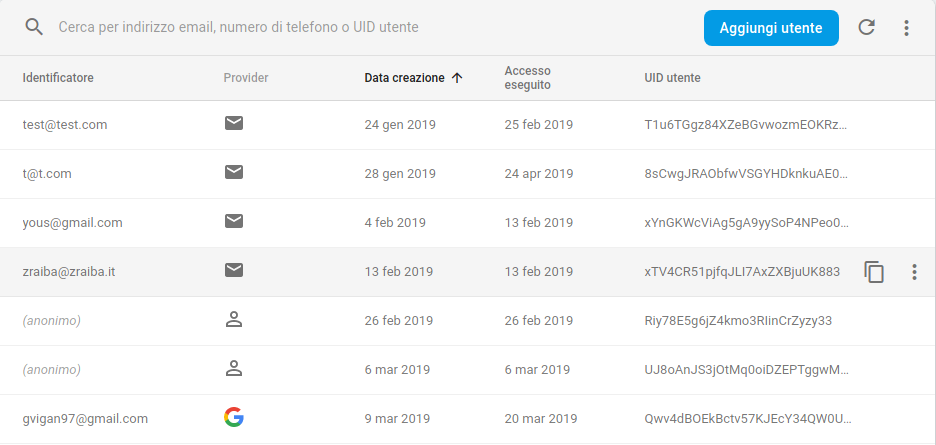
\includegraphics[width=13.5cm]{Authentication.png}
    \caption{La sezione Authentication di Firebase}
    \label{authentication}
\end{figure}

\section{Utente anonimo}
% \subsection{Utente anonimo}
Nella pagina di login è anche possibile premere il tasto "Accedi come Ospite" in
fondo allo schermo, e questo pulsante permette di accedere all'applicazione
senza dover registrare nessun account. La struttura dell'app cambia radicalmente
se si esegue questo tipo di accesso. Innanzitutto sono presenti solo due pagine
accessibili (e non più tre come nel caso di utente standard o Google) e consistono in una
pagina mappa con funzionalità estremamente ridotte e una pagina di Upgrade nella
quale si mostra all'utente i posibili privilegi raggiungibili al momento di
un'autenticazione registrata. Nella sezione \textit{Authentication} del servizo
online di Firebase (figura \ref{authentication}) è possibile prendere visione di tutti gli utenti che hanno
fatto accesso all'applicazione almeno una volta indicando la data di ultima
visita, la data di creazione e l'id dell'utente. Inoltre ne viene indicato anche
il tipo, sia esso account standard, account Google o un utente anonimo.

\section{Codifica}
All'interno del progetto il primo file da cui ha inizio l'esecuzione del codice è il
\textit{main.dart}. Al suo interno è presente il metodo \verb|runApp()| che
prende come argomento l'oggetto che sta a indicare l'intera applicazione e lo esegue.
Per capire lo stato attuale dell'utente all'avvio, cioè per definire se si è già
loggati all'interno dell'app o se è necessario presentare la pagina di login.
Nella seziona di codice seguente si può vedere come sia stata implementata tale
funzione.
\begin{minted}[	frame=lines, framesep=2mm, baselinestretch=1.2,
    fontsize=\footnotesize, linenos	] {python}
@override
void initState() {
super.initState();
if (auth.googleCurrentUser() != null) {
    setState(() {
    _authState = AuthState.signedIn;
    });
} else {
    auth.currentUser().then((user) {
    print(user);
    setState(() {
        if (user == null) {
        _authState = AuthState.notSignedIn;
        } else if (user.isAnonymous) {
        _authState = AuthState.notSignedIn;
        } else {
        _authState = AuthState.signedIn;
        }
    });
    });
}
}
\end{minted}
Tutto il codice è all'interno di initState, la prima funzione
richiamata quando si inizializza l'app. Tramite la variabile \verb|auth| di tipo
Auth (classe implementata all'interno del progetto per rendere facilmente
accessibili le funzionalità dei pacchetti flutter \textit{firebase\_auth} e
\textit{google\_sign\_in}), si controlla subito se l'utente si è gia autenticato
precedentemente con Google. Questo è possibile verificando l'output del metodo
\verb|googleCurrentUser| che restituisce un puntatore all'utente in caso di accesso o
\verb|null| se non è presente nessun utilizzatore. In questo secondo caso, si
verifica quindi che non ci sia già loggati tramite procedura standard tramite
\verb|auth.currentUser|, dal funzionamento molto simile al metodo precedente,
con l'unica differenza che ciò che restituisce è di tipo \emph{Future} e quindi
necessita del metodo then (chiamata asincrona). In base quindi a ciò che viene
restituito si cambia quindi il valore del campo \verb|_authState| tramite un
Enum definito a inizio file con gli unici due stati di loggato (signedIn) e non
loggato (notSignedIn).

	\newpage
	\section{Gestione e struttura del database}

\subsection{Progettazione iniziale}
Una delle prime attività del progetto è stata la progettazione della base di
dati, e fin dall'inizio era chiaro che non si sarebbe trattato di uno schema
molto complesso. Infatti con sole tre tabelle si riesce a descrivere in modo
appropriato l'ambiente nel quale risiede il progetto.
\subsubsection{Schema Concettuale}
 La tabella principale e da cui si è partiti è
quella delle stazioni, che presenta una chiave primaria (Key), un nome con
cui è conosciuta, l'indirizzo cioè il nome della via nella quale risiede, la
posizione, formata da due coordinate geografiche di latitudine e longitudine che
sono realizzate mediante due variabili double, e
può ma non è costretta a possedere una descrizione formata da un testo. La
stazione possiede poi una Tipologia. Tramite colloquio con il commitente dott.
Marco  Aceti si è appreso come le stazioni di ricarica possono essere
raggruppate
in diversi insiemi dovuti al servizio vero e proprio che viene fornito oltre a
quello della ricarica. Esistono stazioni nelle quali è possibile noleggiare bici
elettriche e altre dove si può portare la propria bici per effettuare della manutenzione.
Dunque la tabella TipoStazione contiene per ogni riga una diversa tipologia di
stazione, formata dalla combinazione dei diversi servizi appena descritti, in
quanto ovviamente esistono negozi che propongono più servizi contemporaneamente.
Ogni istanza di questa tabella oltre a possedere una chiave che la identifica,
è caratterizzata dal nome (cioè la tipologia) e da un numero intero chiamato
Colore che viene utilizzato all'interno dell'applicazione per fornire un colore
diverso a ogni tipologia in modo da rendere più semplice agli utenti
l'identiticazione di ciò che può interessare loro. Nello schema deve poi essere
presente una tabella che tenga traccia degli utenti. Si presti attenzione che
questa tabella è diversa da quella gestita da Firebase relativa agli accessi e
alle tipologie di utenti descritta nel precedente capitolo: qui vengono presi in
considerazione il nome dell'utente e oltre alla chiave per identificarlo la
propria preferenza sulla tipologia di mappa scelta. Non si esclude che in futuro
si possano aggiungere ulteriori campi relativi a nuove preferenze che
potrebberero essere scelte. Nella figura \ref{schemaEr} è mostrato lo schema Entità-Relazione
del progetto. Si noti come una stazione debba per forza appartenere alla
relazione Inserimento in quanto deve essere stata inserita da qualcuno, ma un
utente può non appartenere a tale relazione in quanto può tranquillamente
utilizzare l'app per conoscere la posizioni di stazioni senza mai inserirne nessuna.

\begin{figure}[ht!]
    \centering
    {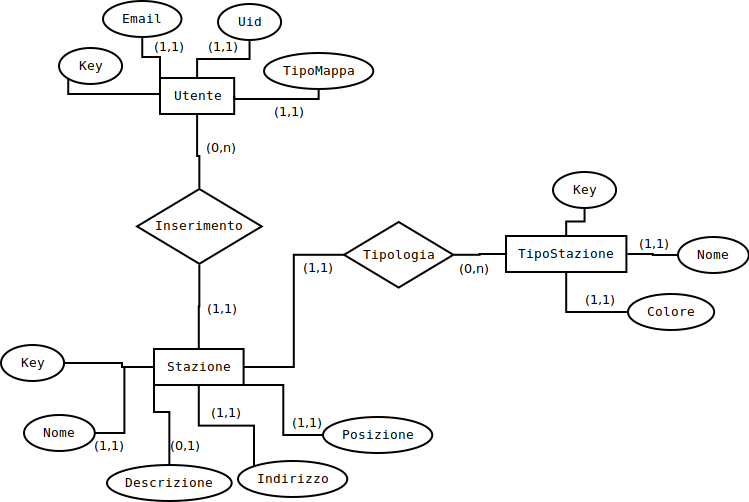
\includegraphics[scale=0.5]{ERTesi.png}}
    \caption{Schema Concettuale del progetto}
    \label{schemaEr}
\end{figure} 

\subsubsection{Schema Logico}
Data la semplicità dello schema Entità-Relazione la fase di progettazione logica
è stata anch'essa priva di ostacoli. Si è posta particolare attenzione alle
relazioni "Inserimento" e "Tipologia" perchè sarebbero potute diventare delle
tabelle ma dato che entrambe sono del tipo (1,1) verso (0,n) si è scelto di
renderle degli attributi della tabella Stazione, diventando quindi chiavi
esterne (figura \ref{schemaLogico}). 

\begin{figure}[ht!]
    \centering
    {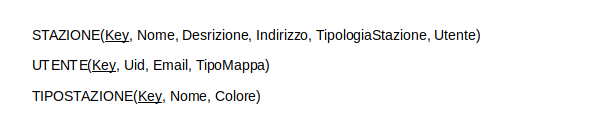
\includegraphics[width=15cm]{LogicoTesi.png}}
    \caption{Schema Logico del progetto}
    \label{schemaLogico}
\end{figure} 

\subsection{Gestione dati in Firebase}
Quando si crea un progetto nella propria Firebase Console una delle prime
importanti operazioni è quella di scegliere la tipologia di database. Il
servizio Google infatti offre due possibili alternative: il Realtime Database
oppure il Cloud Firestore. Fino alla fine del 2018 la prima opzione era anche
l'unica disponibile e consiste in una soluzione efficiente, a bassa latenza per
applicazioni mobili che richiedono la sincronizzazione di stato tra client
diversi in un tempo paragonabile alle prestazioni di un sistema real time. Il
secondo, disponibile da minor tempo, è stato sviluppato per migliorare
ulteriormente il suo predecessore, cambiando anche il modo in cui i dati vengono
organizzati all'interno dello storage. Entrambe queste soluzioni sono database
costruiti per tecnologie NoSQL, dunque non sfruttano le classiche tabelle dove
ogni riga di una tabella è un record che contiene sempre lo stesso numero e
tipologia di attributi. La tipologia Realtime immagazzina i dati in un unico
grande albero JSON. Questo comporta una relativa facilità nell'inseriemento dati
soprattutto se di ridotte dimensioni, ma nel momento in cui la grandezza e
complessità del database non sono più banali diventa difficile organizzare una
struttura gerarchica. La tipologia Cloud immagazzina invece i dati in documenti
chiamati \textit{collections}, ne segue quindi che essa fa parte delle cosiddette
basi di dati oreientate al documento. Strutture dati modeste sono molto facili
da inserire (in modo simile al metodo visto prima tramite JSON) e se queste
diventano complesse e di grandi dimensioni usando collezioni e sotto-collezioni si
può facilmente organizzare il tutto senza perdere in efficienza. Considerando
invece le funzionalità relative all'effettuare query, per il Realtime Database è
possibile filtrare o ordinare dati in una sola query, mentre per il Cloud
Firestore è possibile effettuare entrambe le operazioni nella stessa query.
Inoltre nella prima tipologia il risultato è sempre un albero JSON che contiene
tutti i dati, dunque le dimensioni possono assumere una certa importanza, mentre
nella seconda le performance della query sono proporzionali alla grandezza del
risultato e non dell'intera struttura. A seguito di queste considerazioni si è
quindi deciso, benchè il progetto non presenti strutture particolarmente
complesse, di utilizzare Cloud Firestore. 

\subsection{Utilizzare il Cloud Firestore}
In questa sezione verranno prese in considerazione le modalità con cui si sono
svolte le query all'interno dell'applicazione. Prima di tutto è doveroso dire
che per effettuare interrgoazioni al proprio database è necessario importare nel
proprio progetto il pacchetto \textit{cloud\_firestore}. Grazie a questo si ha
accesso all'oggetto Firestore che permette all'app di comunicare con il database
realtime sul cloud.
\subsubsection{Ottenere tutti gli elementi di una collezione}
Quando si visualizza la pagina della mappa, è necessario visualizzare tutte le
stazioni presenti nel database senza applicare dei filtri. Bisogna quindi
effettuare il corrispettivo di una SELECT ALL nel linguaggio SQL. 
\begin{figure}[!h]
    \centering
    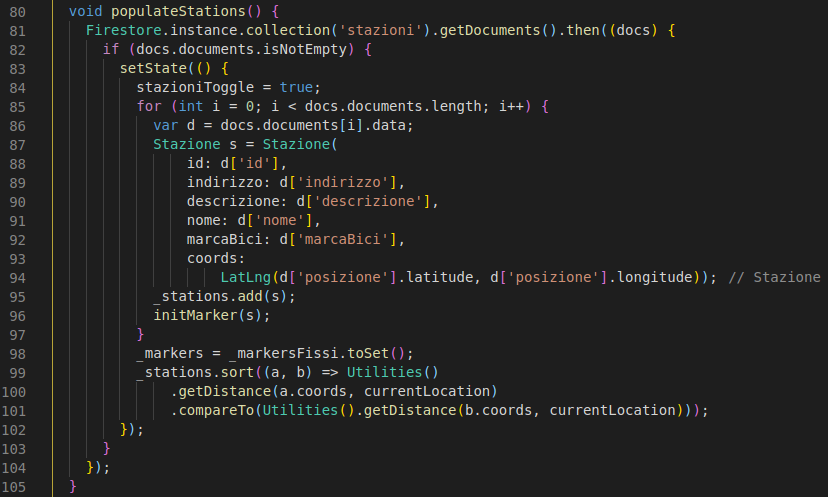
\includegraphics[width=13cm]{query1.png}
    \caption{La funzione populateStations che permette di ottenere tutte le stazioni presenti nel database}
    \label{query1}
\end{figure}
In figura \ref{query1} si può quindi vedere il metodo populateStations che viene
chiamato nel momento in cui l'utente termina la propria autenticazione e
raggiunge la pagina della mappa. Sulla firebase console del progetto è presente
la collezione \textit{stazioni}, a cui si fa accesso alla linea 81 tramite il
metodo \verb|Firestore.instance.collection('stazioni').getDocuments()|. Questo
metodo è di tipo Future (si rimanda al capitolo su Flutter e Dart), e quindi
necessita del metodo \verb|then()| per accedere ai dati inviati in modo
asincrono. Una volta connessi al database e ottenuti i documenti, si controlla
che essi non siano di lunghezza nulla (tramite il campo
\verb|docs.document.isNotEmpty|). Se si è ottenuta almeno una stazione si
procede quindi a creare un oggetto di tipo Stazione per ogni elemento nella
firebase console tramite il suo costruttore, e si inserisce dunque l'oggetto
nella lista di stazioni \verb|_stations|. Si procede poi con la funzione
\verb|initMarker| che inizializza ogni stazione rendendola un marker
visualizzabile nella mappa e si ordinano poi le stazioni in base alla vicinanza
dalla posizione attuale dell'utente tramite una classe (Utilities) creata per
sfruttare funzioni quali l'ordinamento o il controllo di alcuni campi.

\subsubsection{Ottenere dati filtrati da una collezione}
Ci sono diversi casi all'interno dell'applicazione in cui è necessario ottenere
uno specificio documento o un gruppo selezionato da una collezione. Per esempio
per ottenere la preferenza dell'utente rispetto alla tipologia di mappa che
vuole visualizzare bisogna ottenere uno e un solo documento nella collezione
users. \\
\begin{figure}[!h]
    \centering
    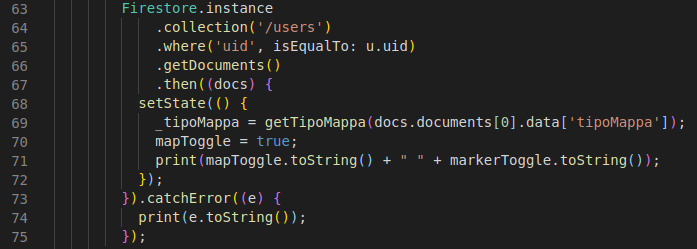
\includegraphics[width=12cm]{query2.png}
    \caption{}
    \label{query2}
\end{figure}
Nella figura \ref{query2} si accede alla collezione users nel solito modo visto
anche precedentemente, ciò che cambia è che ora si introduce anche il metodo
\verb|where()| che prende come primo argomento una stringa indicante il nome del
campo su cui si vuole effettuare la selezione, e un secondo argomento che indica
il tipo di confronto che si vuole fare, in questo caso un \textit{isEqualTo}
(tra gli altri sono presenti anche \textit{isGreaterThan} e
\textit{isLessThan}). Una volta ottenuto l'utente che ha lo stesso id
dell'utser attuale si può quindi accedere al suo campo \verb|tipoMappa| e
tramite un metodo apposito convertire la stringa ottenuta nella tipologia di
mappa desiderata. Si noti anche il metodo \verb|catchError()| che è sucessivo al
\verb|then()| relativo ai documenti della collezione: in caso di un qualunque errore di
connessione l'app non smette di funzionare ma cattura l'eccezione ottenuta e va
avanti nell'esecuzione di codice. Se si volesse effettuare filtraggio di dati su
più campi sarebbe necessario banalmente continuare ad aggiungere metodi
\verb|where| ai documenti ottenuti indicando i nomi dei campi e la condizione
che si vuole applicare.



	\newpage
	\section{Mappa e sue funzionalità}
La pagina della mappa è stata la sezione dell'applicazione più difficile da
implementare, perchè al suo interno risiedono numerosi servizi e funzioni che
hanno richiesto diverso tempo per essere sviluppati e inoltre è stato necessario
documentarsi per capire come utilizzare le API che la pagina utilizza.

\subsection{Scelta del servizio API}
In un primo momento si è pensato di utilizzare il servizio mappe di Google Maps
che, oltre ad essere uno dei più efficienti e meglio documentati, è anche
implementabile facilmente. Il problema è nato nel momento in cui Google ha
deciso di cambiare le proprie politiche di utilizzo delle API verso la fine del
2018. Prima di quel momento, sotto a un certo numero di richieste al servizio di
geolocalizzazione il programmatore poteva usare liberamente il codice e senza
necessità di registrazione, ma in seguito l'azienda di Mountain View ha deciso
che chiunque volesse utilizzare il proprio servizio mappe dovesse prima
registrare un proprio account ed inserire una carta di credito che eventualmente
pagasse mensilmente le risorse di cui si è fatto uso. Questo scenario ha portato
a prendere in cosiderazione altri gestori di mappe. La scelta è ricaduta su
MapBox, azienda emergente nel proprio campo. Il servizio era gratuito e permetteva
un agevole utilizzo senza registrazione ma il problema era formato
dall'implementazione vera e propria. Al contrario di Google, non esiste un
pacchetto software che implementi il codice MapBox e quindi era necessario fare
uso di richieste http tramite valori codificati all'interno di lunghi url.
Inoltre la fluidità della mappa non rispettava le direttive del committente
dott. Marco Aceti, spesso a seguito di un rapido movimento delle dita per
spostarsi in un'altra zona della mappa la schermata rimaneva per qualche secondo
completamente grigia, rendendo l'esperienza di utilizzo sicuramente peggiore.
Nel seguito, tra Gennaio e Febbraio 2019 è stata rilasciata la prima versione
ufficiale di Flutter (versione 1.0.0) e tra le tante novità spiccava la presenza
di un widget particolare, chiamato GoogleMap. Semplificando notevolmente
l'utilizzo delle mappe, tale widget presenta ottime prestazioni e facilità di
implementazione. Si è quindi deciso di dedicare del tempo nell'apprendere ogni
aspetto delle politiche di utilizzo delle API di Google, capendo quindi che,
facendo un numero di richieste minore di una soglia stabilita, non è necessario
pagare nulla, anche se si è registrata una carta di credito. Quindi la scelta è
ricaduta sulle API di Google e si è importato nel progetto il pacchetto
\verb|googlemap|.

\subsection{MapPage}
Dopo che l'utente ha eseguito correttamente la procedura di login o ha aperto
l'applicazione in caso di autoidentificazione con mantenimento dello stato della
registrazione, viene mostrata la MapPage. In alto è presente un'AppBar che 
mostra il titolo eBike-Recharge, in basso è presente una TabBar che permette di
navigare tra le pagine dell'app. Tra le due, a tutto schermo, viene mostrata la
mappa con al centro la posizione attuale dell'utente. Quest'ultima può essere di
diversi tipi a seconda delle preferenze indicate nella pagina profilo
dell'utilizzatore. In particolare si può scegliere tra \textit{Normale}, cioè la
classica modalità di visualizzazione di mappe che viene mostrata di default
sull'app Google Maps, \textit{Rilievo}, dove è presente l'altitudine delle
montagne indicata con diversi colori in base all'altezza, mancando però
di indicare i nomi di edifici importanti, negozi o imprese, \textit{Satellite},
che mostra con una serie di foto satellitari i luoghi indicati dall'alto, in
modo da vedere realmente il percorso che si deve intraprendere
per raggiungere la propria destinazione, e \textit{Ibrida}, che può essere
considerata l'unione di Satellitare e Normale, poichè oltre a presentare
l'altitudine mostra anche i nomi dei luoghi di maggior importanza della zona
visualizzata.

\begin{figure}[h!]
    \centering
    \begin{subfigure}{0.33\linewidth}
        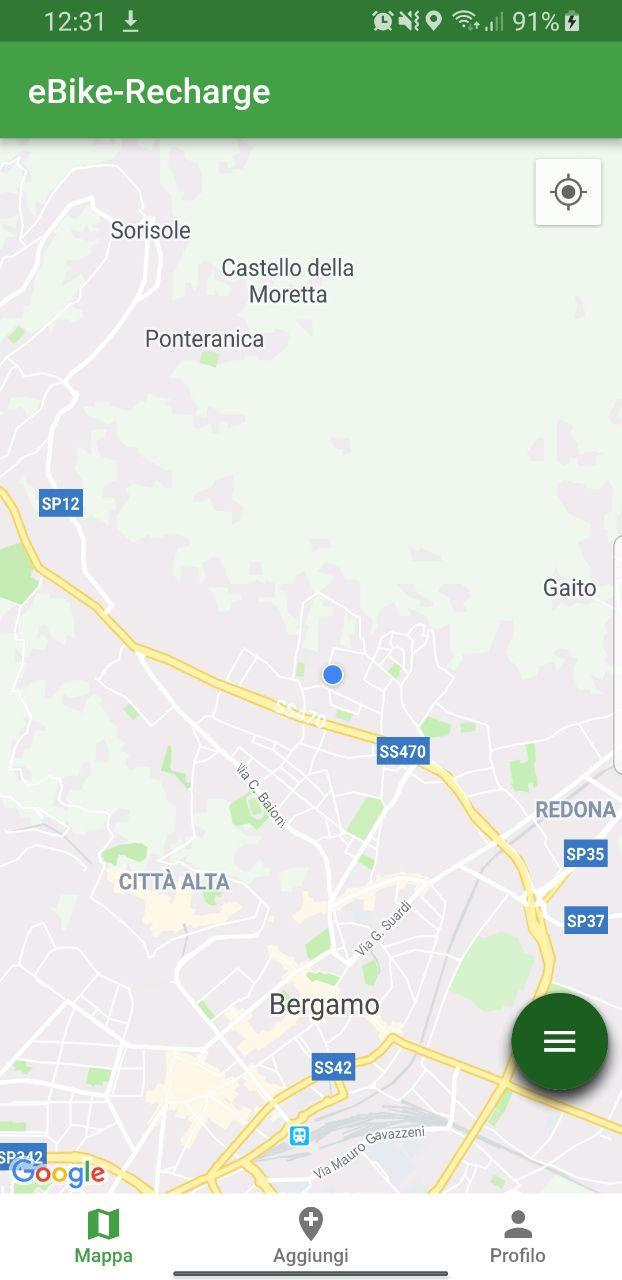
\includegraphics[width=\linewidth, height=9cm]{MapNormale.jpg}
        \caption{Normale}
    \end{subfigure}
    \begin{subfigure}{0.33\linewidth}
        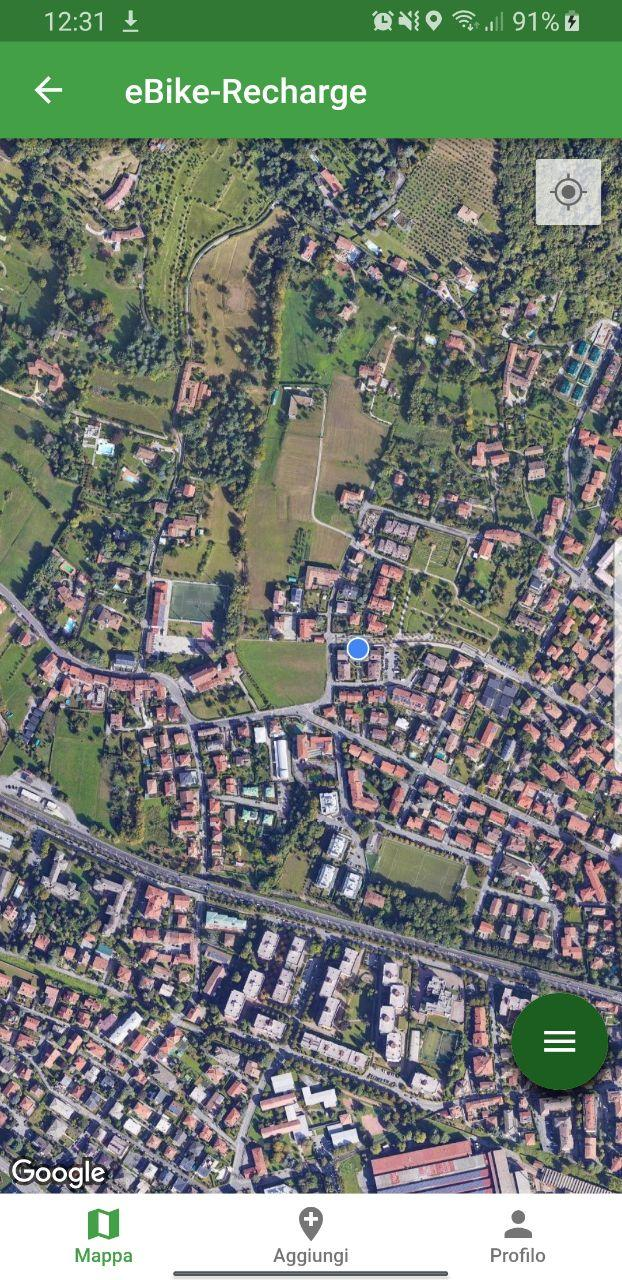
\includegraphics[width=\linewidth, height=9cm]{MapSatellite.jpg}
        \caption{Satellite}
    \end{subfigure}
    \begin{subfigure}{0.33\linewidth}
        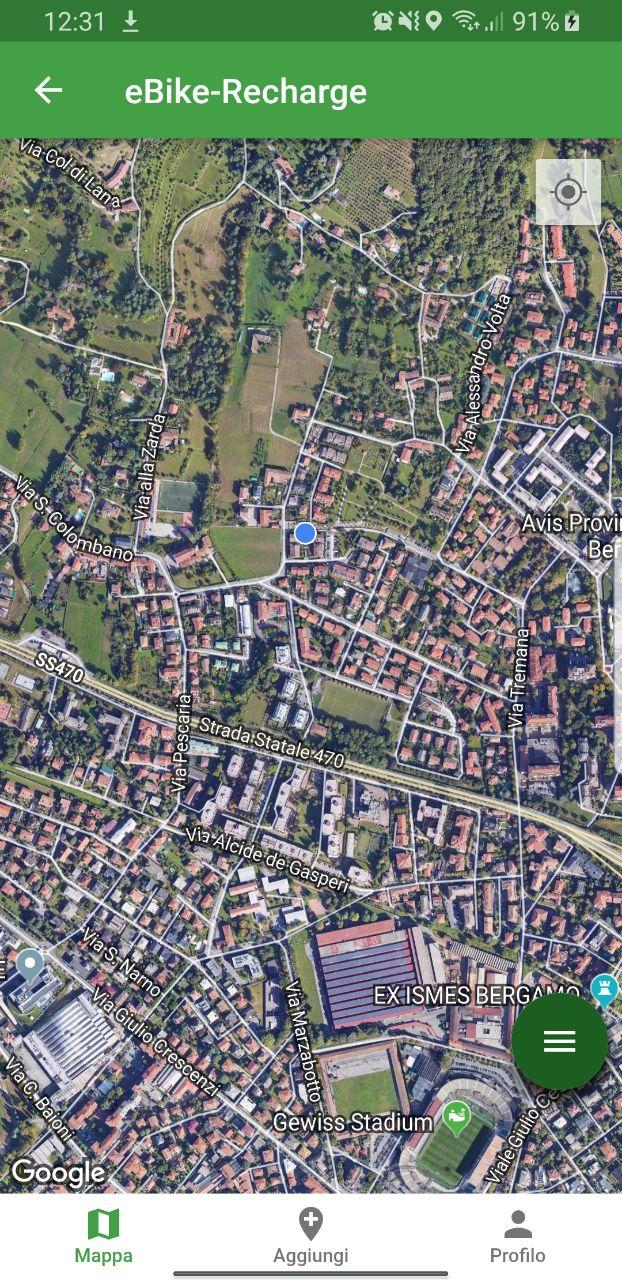
\includegraphics[width=\linewidth, height=9cm]{MapIbrida.jpg}
        \caption{Ibrida}
    \end{subfigure}
    \begin{subfigure}{0.33\linewidth}
        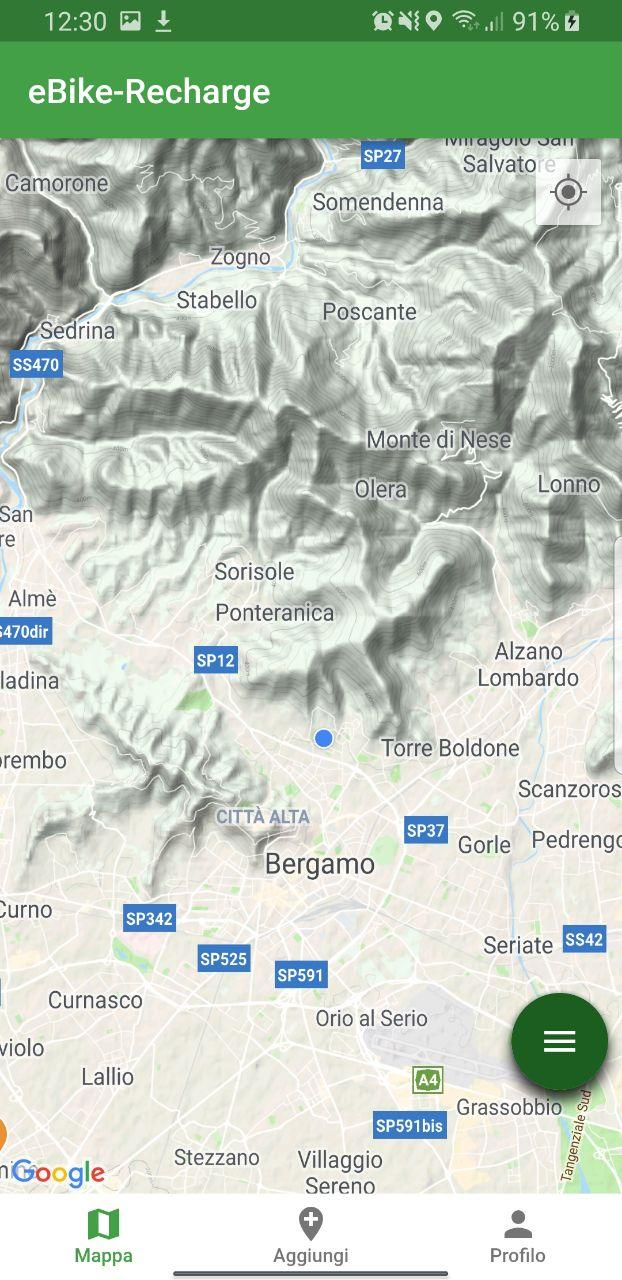
\includegraphics[width=\linewidth, height=9cm]{MapRilievo.jpg}
        \caption{Rilievo}
    \end{subfigure}
    \caption{I quattro tipi di mappa selezionabili nella pagina profilo}
    \label{TipoMappa}
\end{figure} 

Grazie al pacchetto googlemap di flutter si è riusciti a implementare un oggetto
GoogleMap (che verrà descritto in un successivo paragrafo) con cui è molto
facile interagire. In particolare, l'utente può aumentare o diminuire lo zoom
della mappa con i classici gesti di allontanamento o avvicinamento delle dita, e
può spostarsi in diverse zona semplicemente trascinando verso la direzione
desiderata. Con una buona o anche solo media connessione internet i tempi di
latenza sono pressochè nulli, così che non si riesca a vedere i riquadri grigi
che il widget crea nel momento in cui si cambia direzione e che dovranno essere
riempiti con le nuove località. Questi ultimi sono pienamente visibili nel
momento in cui non si disponga di una connessione adeguata, condizione che si
verifica sempre più di rado negli ultimi tempi. 


\subsection{Funzionalità}
Nelle immagini precedenti si è forse notato un pulsante nella parte inferiore
dello schermo verso destra. Se toccato (figura \ref{4puls}), quest'ultimo mostra una serie di
pulsanti con diverse funzionalità. 
\begin{figure}
    \centering
    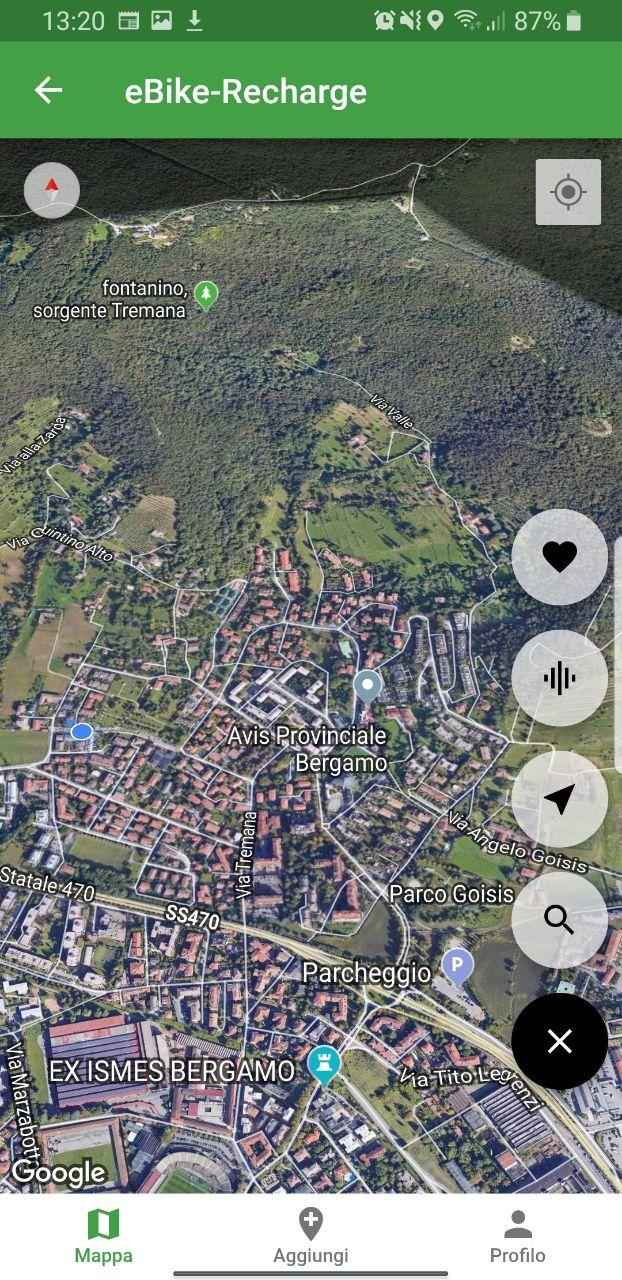
\includegraphics[width=7cm]{MapFun.jpg}
    \caption{Premuto il pulsante, vengono mostrati i 4 FloatingActionButton e il quinto (con la X) per tornare indietro}
    \label{4puls}
\end{figure}
Il primo è un'icona a forma di cuore e,
interagendo con esso, viene mostrato un BottomSheet (spiegato nel secondo
capitolo, Flutter) che mostra una Card (una piccola scheda con titolo e icona)
con le stazioni di ricarica preferite dall'utente. Per esprimere la propria
preferenza per una stazione è necessario entrare nella scheda di quest'ultima e
selezionare il cuore presente in alto a destra. \\
Il secondo pulsante ha la funzione di filtro e al tempo stesso di legenda.
Premendolo, viene mostrata a schermo una AlertDialog (fig. \ref{filtro}) che indica quali
tipologie di stazioni si desidera cercare. Sulla destra sono presenti dei Button
di tipo check (che possono essere True o False): se si vede la casella spuntata
allora si vedra la relativa tipologia sulla mappa, se tale casella è vuota
allora la mappa verrà filtrata e non sarà possibile cercare tutte le stazioni di
quel tipo. \\
Il terzo pulsante mostra un'icona con la classica freccia indicante la
navigazione e, se premuto, fa apparire un BottomSheet con Card contenente le
dieci stazioni più vicine alla posizione attuale dell'utente. Come per tutte le
Card anche nelle altre funzionalità, è possibile definire un'azione in seguito
al tocco della scheda. In seguito all'interazione dell'utilizzatore con una
specifica Card, la mappa ruota e cambia il proprio centro mostrando l'icona
indicante quella stazione che si è toccata. In questo modo l'utente risparmia
tempo poichè viene direttamente condotto alla stazione di interesse.
\begin{figure}[h!]
    \centering
    \begin{subfigure}{0.3\linewidth}
        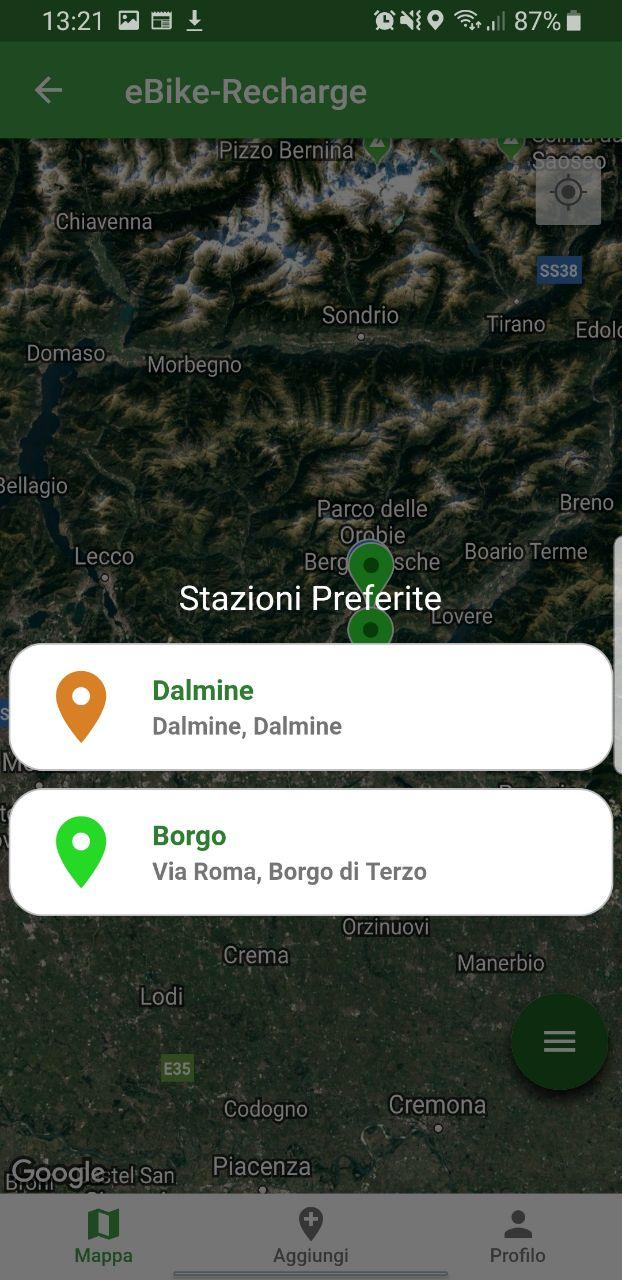
\includegraphics[width=\linewidth, height=9cm]{MapFunFavourite.jpg}
        \caption{Preferiti}
    \end{subfigure}
    \begin{subfigure}{0.3\linewidth}
        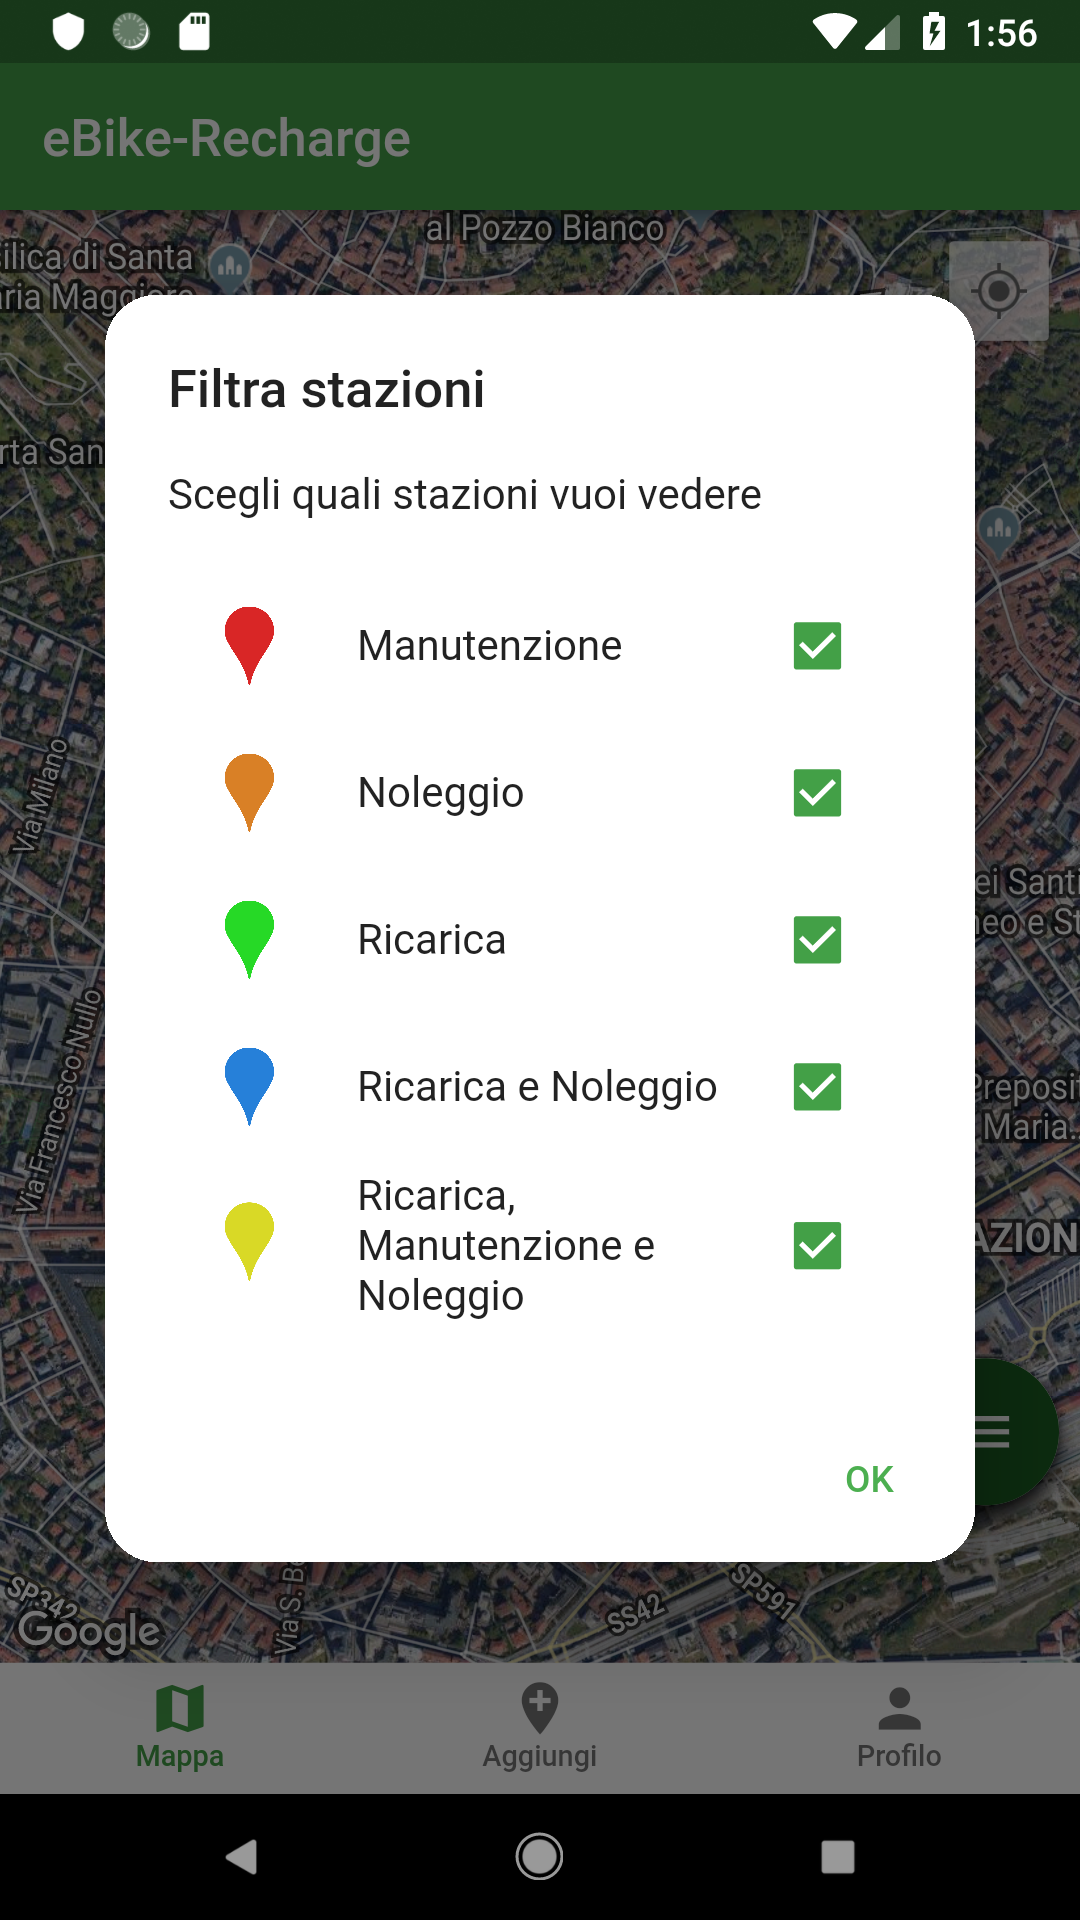
\includegraphics[width=\linewidth, height=9cm]{MapFunFilter.png}
        \caption{Filtro e Legenda}
        \label{filtro}
    \end{subfigure}
    \begin{subfigure}{0.3\linewidth}
        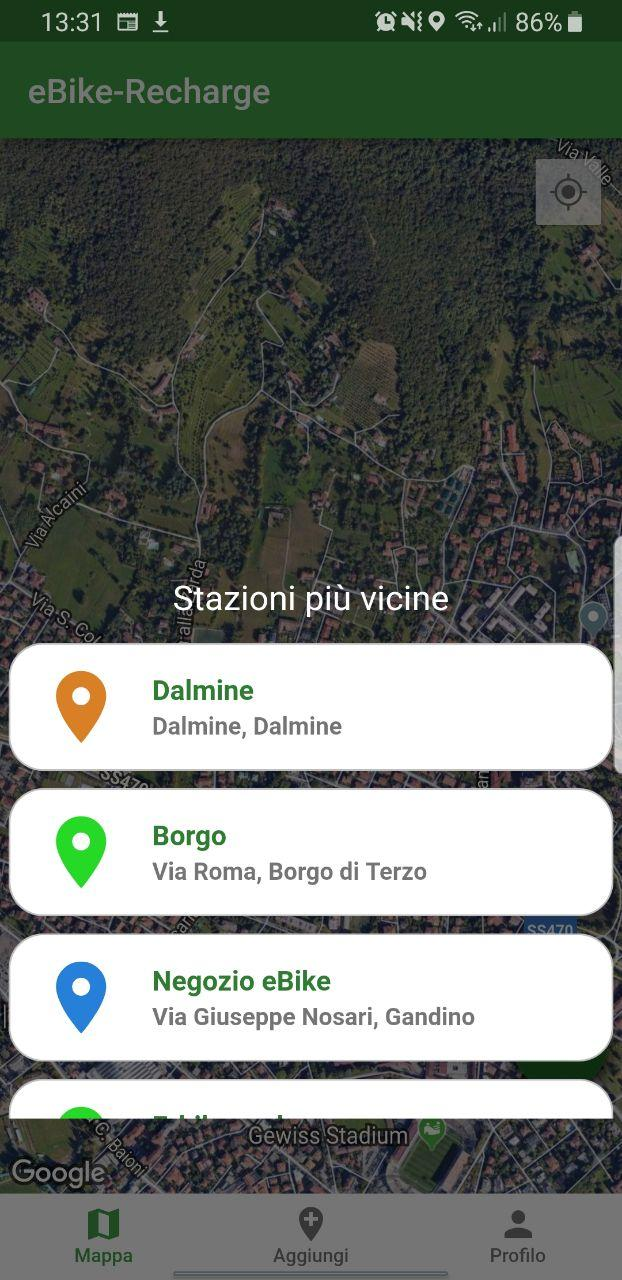
\includegraphics[width=\linewidth, height=9cm]{MapFunNearest.jpg}
        \caption{Stazioni più vicine}
    \end{subfigure}
    \caption{}
\end{figure}

L'ultimo pulsante è accompagnato da un'icona rappresentante una lente di
ingrandimento, simbolo universale di ricerca. Premendolo, in alto sullo schermo
appare un TextField con impresso la frase "Cerca Indirizzo". L'utente è quindi
invitato a digitare la via o la località che desidera vedere. Mentre si forma la
scritta, grazie al servizio API Google Places l'app è in grado di mostrare
diverse Card a schermo con suggerimenti, fungendo quindi da auto-completamento.
Se l'utente clicca su una di queste sezioni viene richiamata la stessa funzione
delle Card prima mostrata: la mappa cambia centro e porta l'utente nella via
desiderata. Questo servizio costa una frazione di centesimo per ogni singola
chiamata alla funzione di auto-completamento. Si è quindi deciso di introdurre
un limite mensile al numero di volte che l'app può far uso di questa API, in
corrispondenza del numero massimo di chiamate che si possono fare senza dover
pagare direttamente Google.
\begin{figure}[h!]
    \centering
    \begin{subfigure}{0.33\linewidth}
        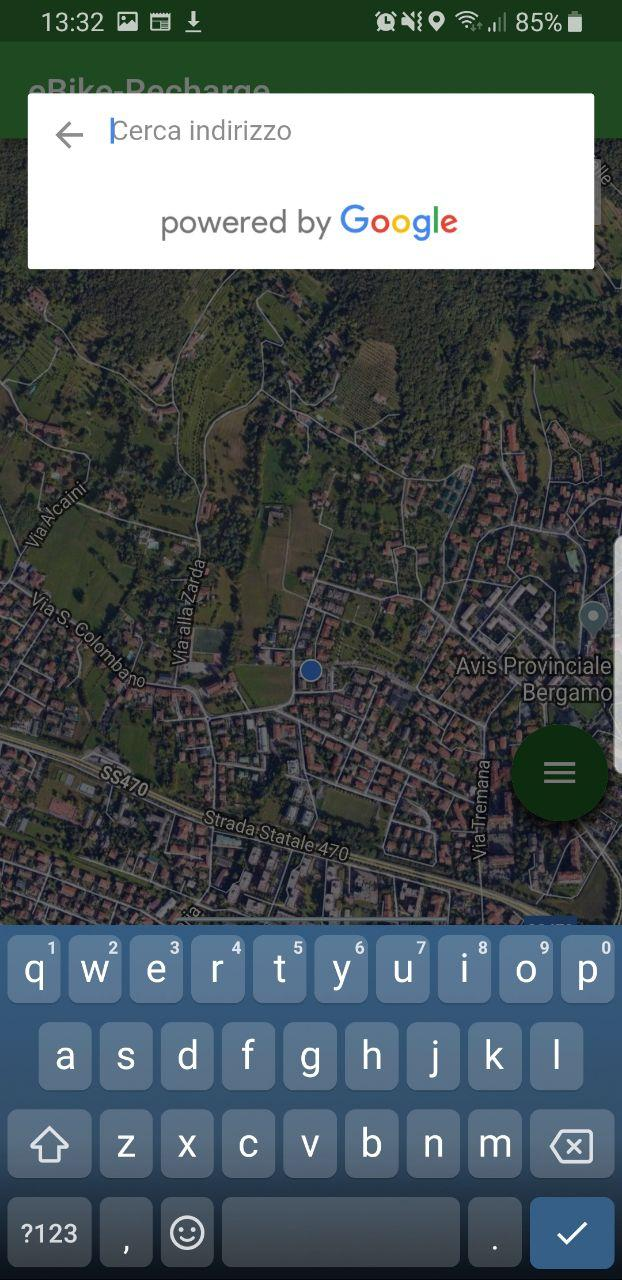
\includegraphics[width=\linewidth, height=9cm]{MapFunSearch1.jpg}
    \end{subfigure}
    \begin{subfigure}{0.33\linewidth}
        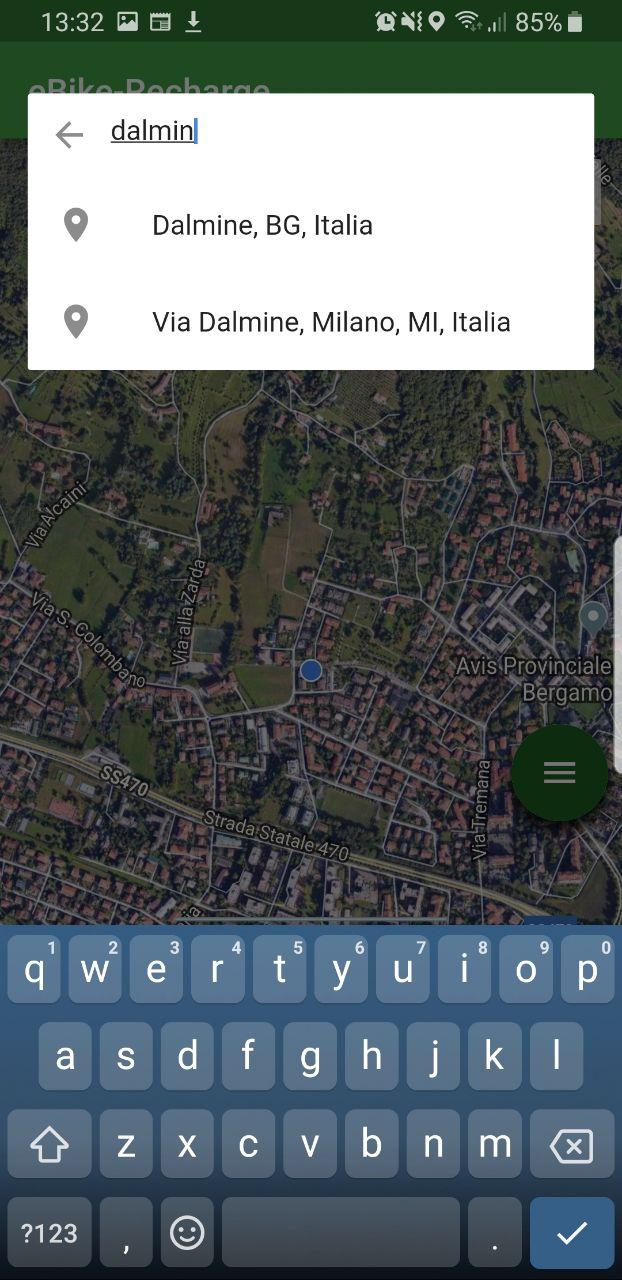
\includegraphics[width=\linewidth, height=9cm]{MapFunSearch2.jpg}
    \end{subfigure}
    \caption{La funzione di ricerca e autocompletamento dell'API Google Places}
\end{figure}

\subsection{Aggiungere una Stazione}
	
\end{spacing}

	
	
	\bibliographystyle{plainnat}
	% bibliografia
	\newpage
	\bibliography{bibliografia}
\end{document}